\documentclass[11pt,a4paper]{article}
\usepackage{a4wide}
\usepackage{enumerate}
\usepackage{enumitem}
\usepackage{pcptex}
\usepackage{xspace}
\usepackage[toc,page]{appendix}

\graphicspath{{figures/}}
\usepackage{subcaption}
\usepackage{algorithm}
\usepackage[noend]{algpseudocode}

\usepackage[font=small,labelfont=bf,tableposition=top]{caption}

% ref packages
\usepackage{nameref}
% folowing  must be in this order
\usepackage{varioref}
\usepackage{hyperref}
\usepackage{cleveref}

%\usepackage{wrapfig}
\usepackage[utf8]{inputenc}
\usepackage{pgfplots}
%\usepgfplotslibrary{plotmarks}
\newlength{\figureheight}
\newlength{\figurewidth}

\makeatletter
\def\BState{\State\hskip-\ALG@thistlm}
\makeatother

\begin{document}

\pptitle{A High Performance Implementation of the Escape Time Algorithm to generate the Mandelbrot Set}

\vspace{-1.1cm}
\ppintro{Concetto Emanuele Bugliarello}{EPFL}{/}{Only PI}{\today}{June 4, 2017}{Deneb}{MNDLBRT}

\vspace{-1.3cm}
\ppabstract{
The Mandelbrot set is at the heart of fractal-like structures and many people have generated breathtaking drawings by sampling the complex numbers in it.
In this project, we present a parallel implementation of the \textquotedblleft escape time\textquotedblright~algorithm, one of the algorithms used to produce such drawings.
Our application is coded in C and makes use of the MPI standard and the CUDA platform.
The source code is available in the c4science repository at: \url{https://c4science.ch/diffusion/3860/mndlbrt.git}
}


\section{Scientific Background}

The Mandelbrot set is the set of complex numbers $c$ for which the function $f_{c}(z)=z^{2}+c$ does not diverge when iterated from $z=0$~\cite{wiki:mandelbrot}.
That is, if we denote the Mandelbrot set by $M$, then by repeatedly applying the quadratic map
\[
\left\{
\begin{array}{ll}
z_0 = 0\\
z_{n+1} = z_n + c,
\end{array}
\right.
\]
for any complex number $c$, we have that $c\in M\iff\limsup _{n\to \infty }|z_{n+1}|\leq 2$.\\

To generate Mandelbrot set images, we can sample the complex numbers and iterate this function for each point $c$ that has been sampled.
If the function goes to infinity, then the point belongs to the set.
Each sampled point can then be represented on a 2D plane by treating its real and imaginary parts as image coordinates $(x+yi)$ and coloring the corresponding pixel according to how quickly the sequence $z_{n}^2 + c$ diverges.\\
Two examples of such representation are shown in Figure \ref{fig:both-mandelbrot}.
In particular, points belonging to the set are colored in black, while points not in the set are colored according to how many iterations are required for the absolute values of the corresponding sequences to become greater than a cutoff value (2).\\
\begin{figure}[t]
	\vspace{-0.5cm}
	\centering
	\begin{subfigure}{.35\textwidth}
		\centering
		\includegraphics[width=.95\linewidth, clip, trim={3cm 0cm 2cm 0cm}]{red.pdf}
		\caption{Red-shaded drawing.}
		\label{fig:mandelbrot-red}
	\end{subfigure}%
	\begin{subfigure}{.35\textwidth}
		\centering
		\includegraphics[width=.95\linewidth, clip, trim={3cm 0cm 2cm 0cm}]{blue.pdf}
		\caption{Smooth, blue-shaded drawing.}
		\label{fig:mandelbrot-blue}
	\end{subfigure}
	\vspace{-0.3cm}
	\caption{Mandelbrot set drawings generated with our palettes.}
	\label{fig:both-mandelbrot}
\end{figure}

There exist many algorithms to draw the Mandelbrot set. 
Since our goal is to produce a parallel implementation in CUDA~\cite{cuda} and MPI~\cite{mpi}, we use one of the simplest algorithms to generate a pictorial representation of the Mandelbrot set: the \textquotedblleft escape time\textquotedblright~algorithm.
In fact, this algorithm results in an embarrassingly parallel problem: each pixel does not depend on any other, allowing each thread in the GPU to run its computations independently and avoiding exchanging ghost cells when MPI is used.
The pseudocode of this algorithm follows.\\
\setlength{\textfloatsep}{6pt} % Space after algorithm
\begin{algorithm}
	\caption{Escape Time algorithm}\label{euclid}
	\begin{algorithmic}[1]
%		\Procedure{}{}
		\For {each pixel (Px, Py) on the screen}
		\State $x_0 \gets$ scaled x coordinate of pixel
		\State $y_0 \gets$ scaled y coordinate of pixel
		\State $x \gets 0.0$
		\State $y \gets 0.0$
		\State $iteration \gets 0$
		\While {$(x\times x + y\times y < 2\times 2$  AND  $iteration < max\_iteration)$}
			\State $x_{temp} \gets x\times x - y\times y + x_0$
			\State $y \gets 2\times x\times y + y_0$
			\State $x \gets x_{temp}$
			\State $iteration \gets iteration + 1$
		\EndWhile
		\State $color \gets palette[iteration]$
		\State $plot(Px, Py, color)$
		\EndFor
%		\EndProcedure
	\end{algorithmic}
\end{algorithm}
\noindent
Where $z = x + iy$, $c = x_0 + iy_0$, $x = Re(z^2+c)$ and $y=Im(z^2+c)$.\\
Note that we keep iterating up to a fixed number of steps.
Hence, we decide that a sampled point is \textquotedblleft probably\textquotedblright~in the Mandelbrot set after $max\_iteration$ iterations.

\vspace{-0.3cm}
\section{Implementations}

The application is coded in C~\cite{ritchie} and three main classes of implementations are developed:
\begin{itemize}
\vspace{-0.2cm}
\itemsep0em 
	
\item Serial versions.
\item GPU versions using the CUDA parallel computing platform.
\item Hybrid versions using both CUDA and MPI (including MPI-IO).
\end{itemize}
\vspace{-0.1cm}
The code has been fully debugged using the \texttt{gdb} debugger. 
The \texttt{Valgrind} tool has been used to make sure that all heap blocks are freed and hence no memory leaks are possible. 

\vspace{-0.3cm}
\subsection{Serial implementations}

We start by implementing a naive version of the described algorithm and two plotting functions: a simple one with a red hue (Figure \ref{fig:mandelbrot-red}), and a smoother version in blue\footnote{It uses an approximation of the Normalized Iteration Count method presented in \cite{smooth}.} (Figure \ref{fig:mandelbrot-blue}).
While the latter is prettier, it needs the real and imaginary values reached by each pixel in the quadratic map, thus requiring, in a first implementation, the allocation of two additional matrices of doubles (one for the real and one for the imaginary parts) of the same size as the total number of pixels.
Throughout this project, we produce smooth, blue drawings as in Figure \ref{fig:mandelbrot-blue}.\\[-7pt]
\begin{table}[t]
	\vspace{-0.5cm}
	\begin{minipage}[b]{0.4\linewidth}
		\centering
		\frame{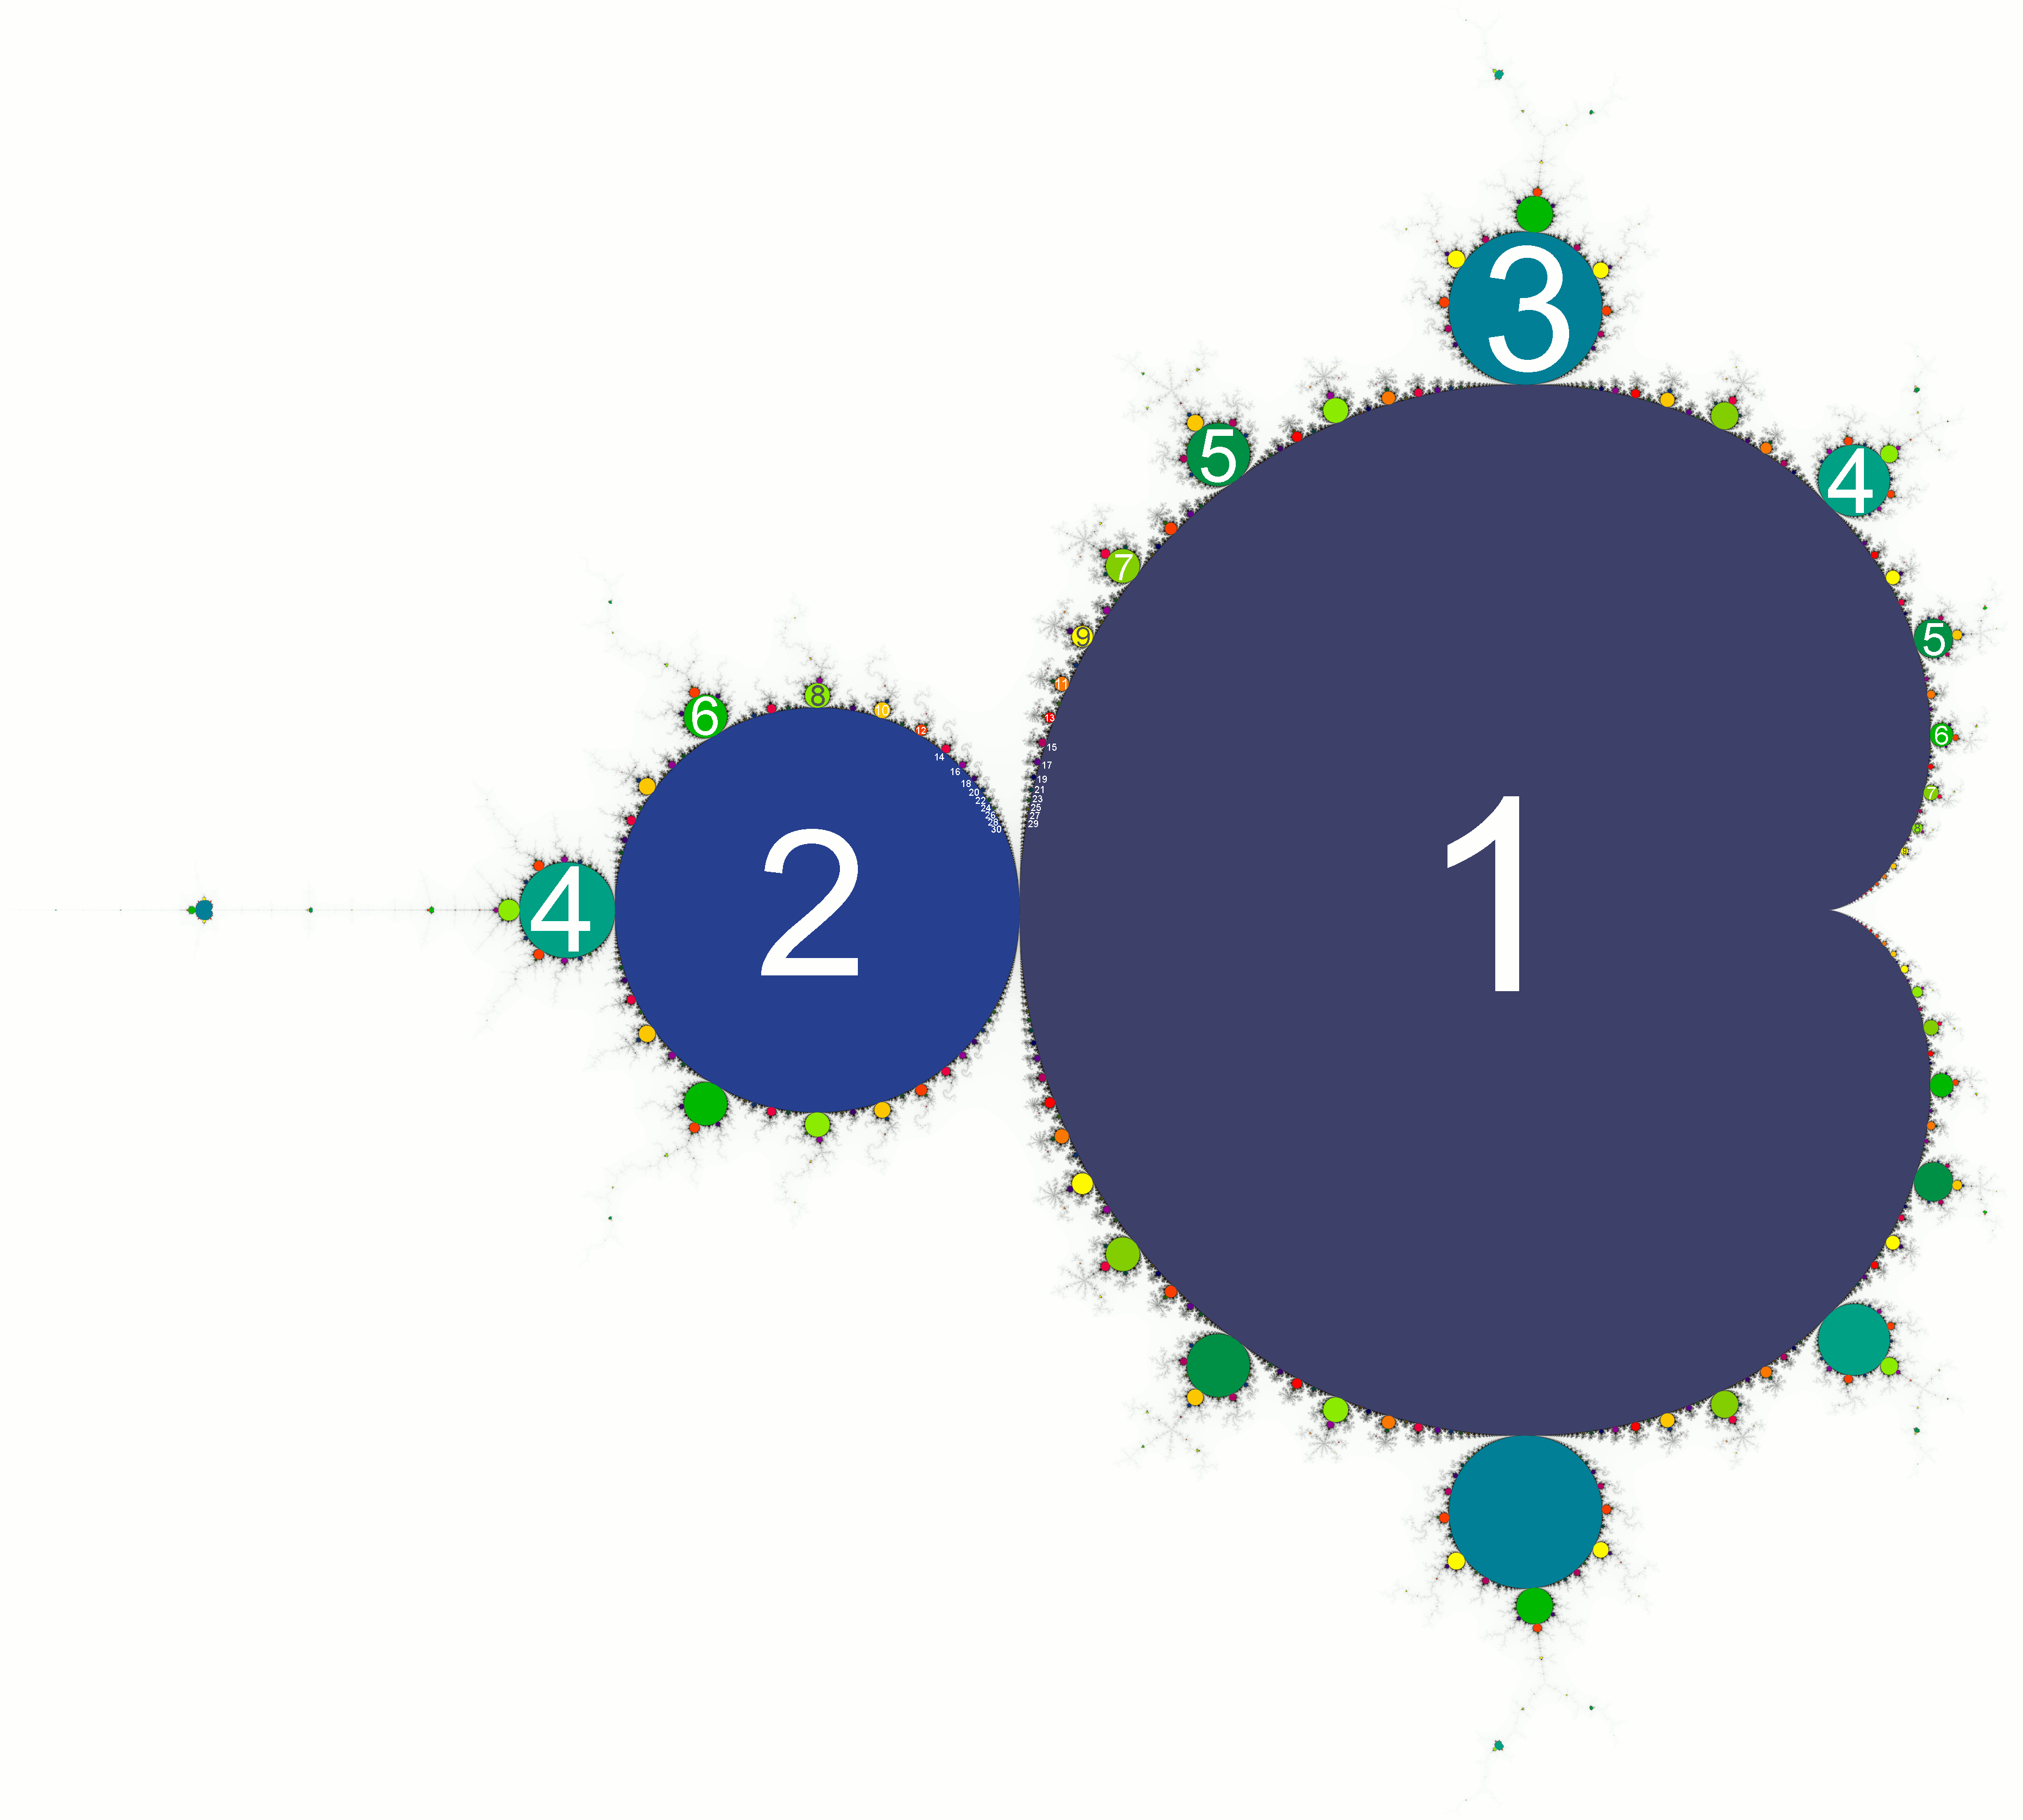
\includegraphics[width=0.565\textwidth]{bulbs.png}}
		\vspace{0.2cm}
		\captionof{figure}{Periods of hyperbolic components~\cite{wiki:mandelbrot}.} \label{fig:bulbs}
	\end{minipage}\hfill
	\begin{minipage}[b]{0.56\linewidth}
		\centering
		\begin{tabular}{|l|l|} 
			\hline
			\textbf{Optimization level} & \textbf{Execution time [s]} \\ [0.2ex] 
			\hline\hline
			\texttt{-O0} & 422.91 \\ 
			\texttt{-O1} & 230.99 \\
			\texttt{-O2} & 208.96 \\
			\texttt{-O3} & 208.49 \\
			\texttt{-O3 -ftree-vectorize} & 205.41 \\ [0.2ex] 
			\hline
		\end{tabular}
		\vspace{0.2cm}
		\caption{Execution times of \texttt{opti3} for a $25600\times14400$-pixel image and $max\_iteration=10,000$ as a function of the optimization level.}
		\label{tab:opti-levels}
		\vspace{-0.2cm}
	\end{minipage}
\end{table}

\noindent
Beside the standard optimizations (such as vectorization), we exploit the characteristics of the problem at hand in order to further improve the performance.\\[-7pt]

Firstly, as we can see from the pictures above, the resulting figure is symmetric with respect to the $x$ axis.
Then, we only compute the values for half of the specified height and fill the other half of the image during the plotting phase.
We refer to this first optimization as \texttt{opti1}.\\[-7pt]

Secondly, it is possible to skip the calculations for the points lying within the cardioid or in the period-2 bulb (marked with 1 and 2, respectively, in Figure \ref{fig:bulbs}).
 
%\begin{figure}
%	\vspace{-0.2cm}
%	\centering
%	\frame{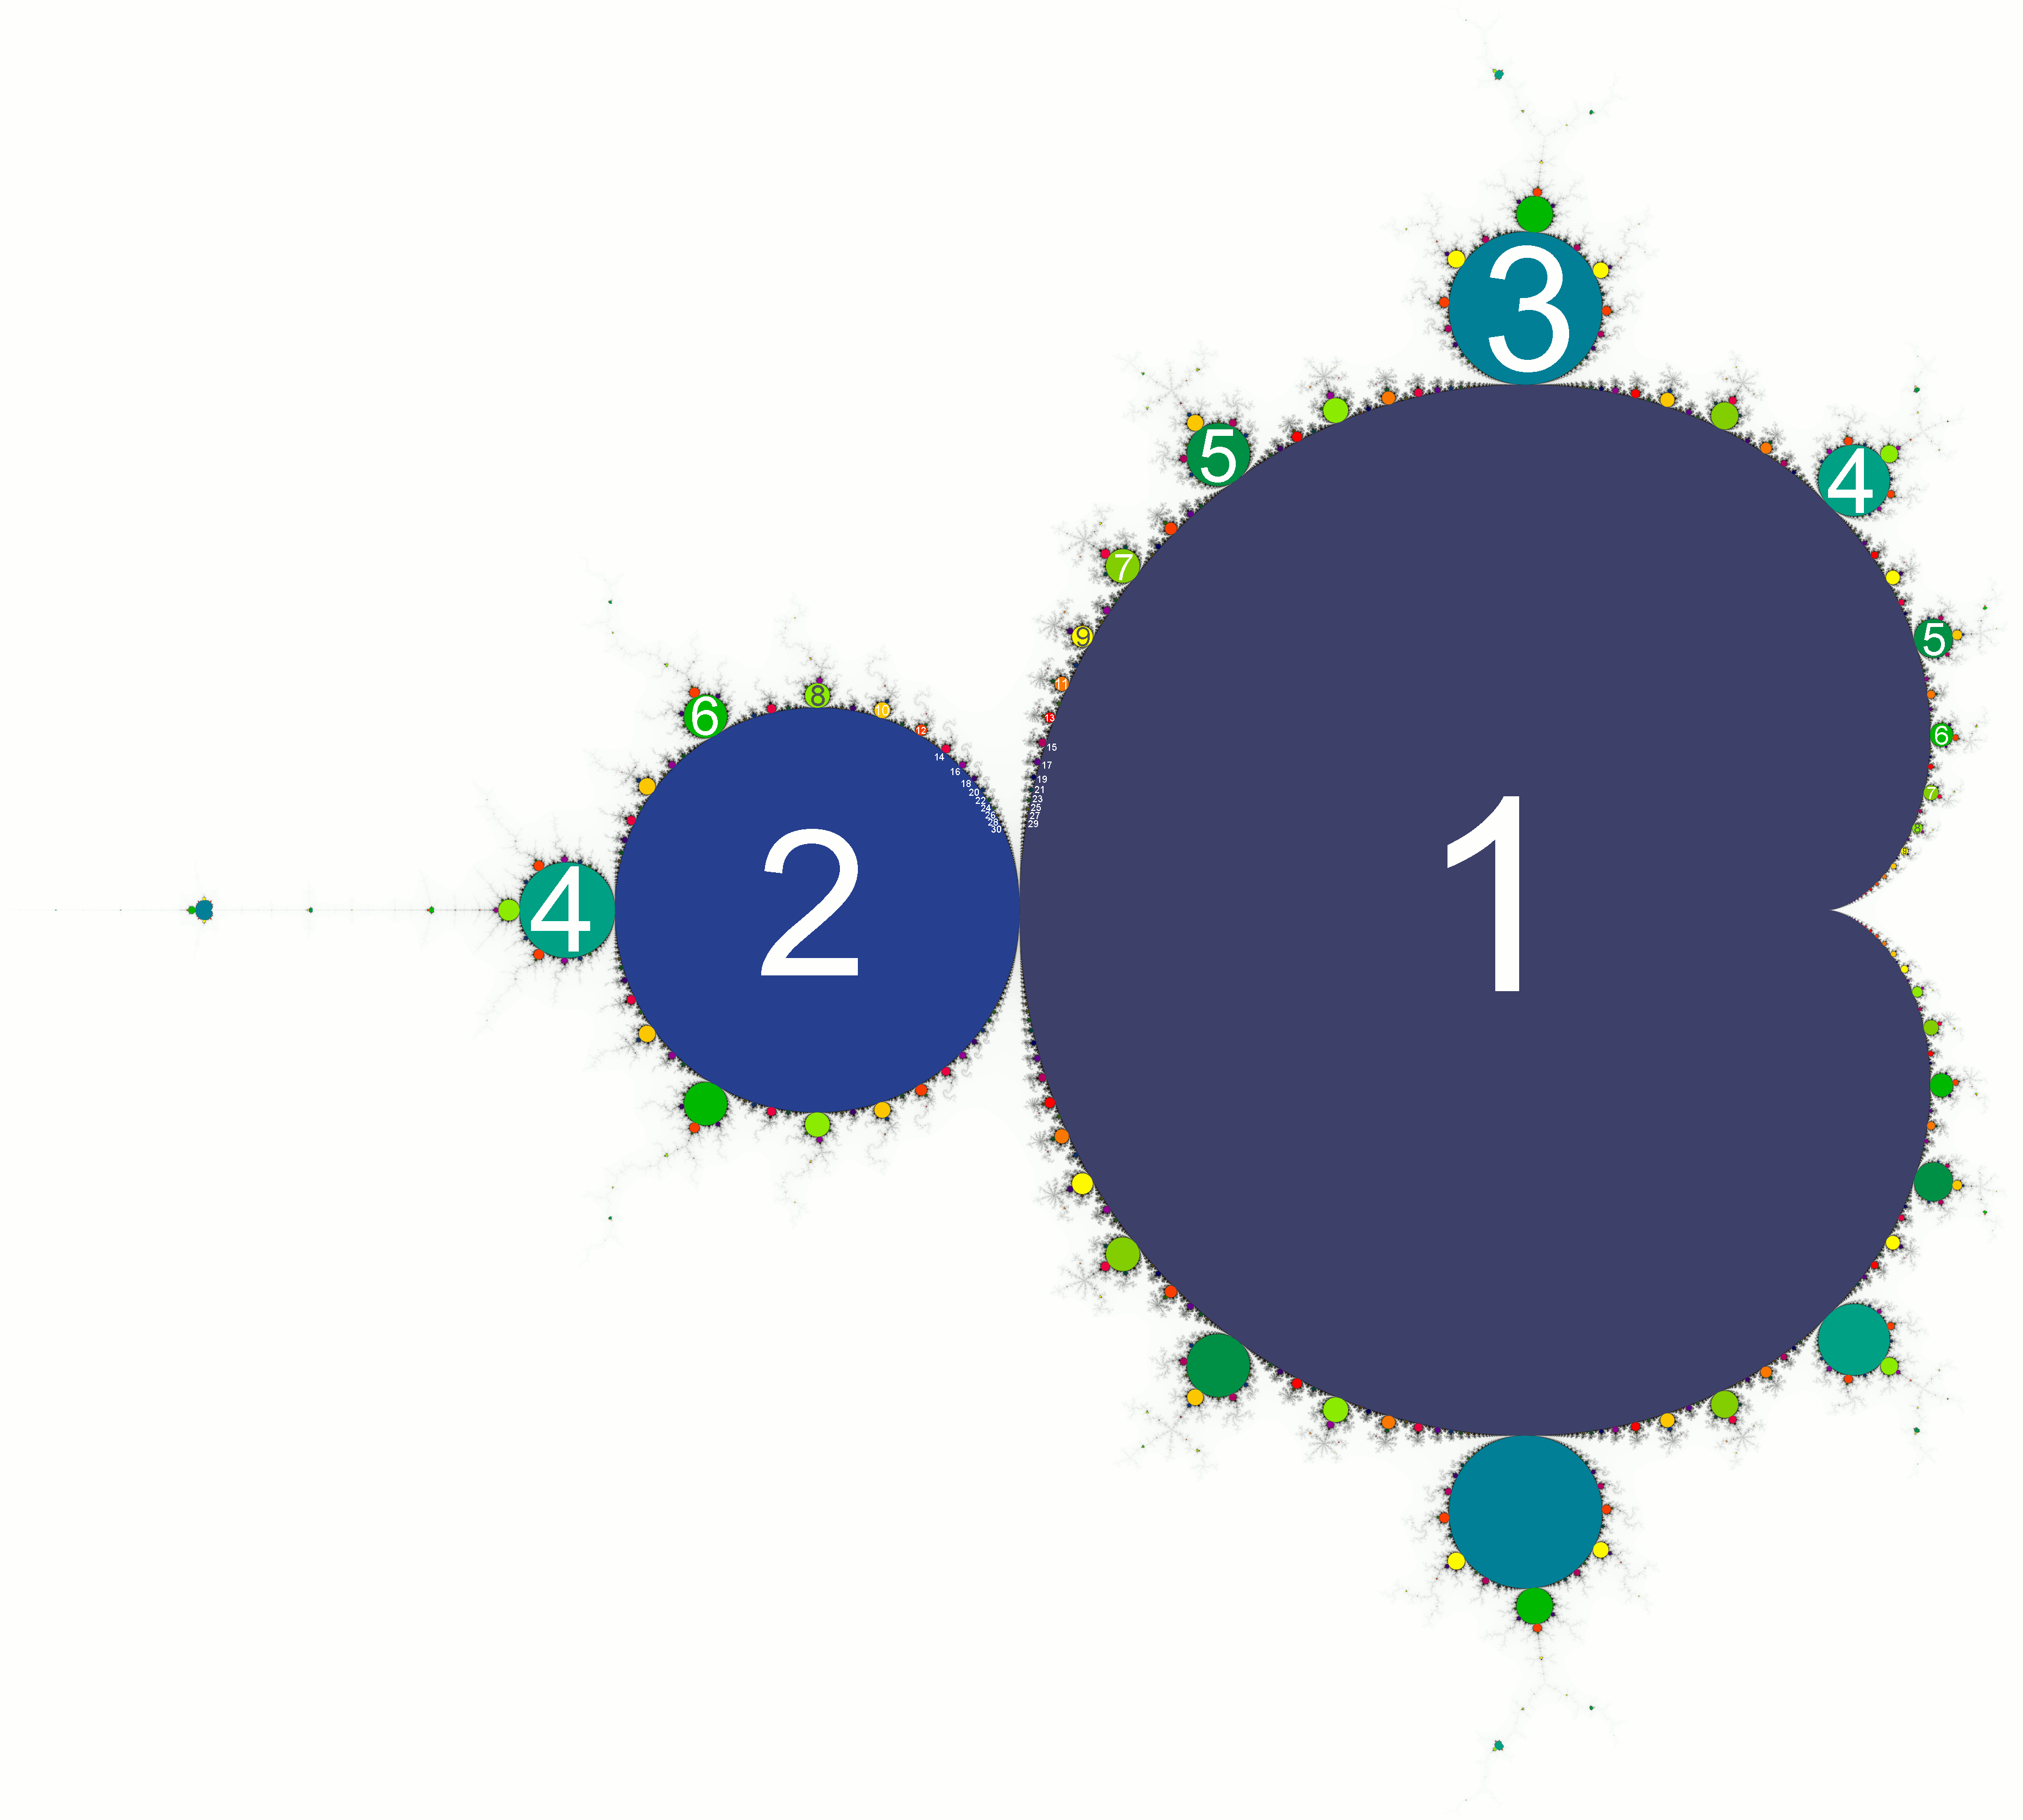
\includegraphics[width=0.2\textwidth]{bulbs.png}}
%	\caption{Periods of hyperbolic components~\cite{wiki:mandelbrot}.} \label{fig:bulbs}
%	\vspace{-0.1cm}
%\end{figure}
\noindent
To do so, before passing a point to the escape time algorithm, we first check whether one of the following equations hold:
\[
\left\{
\begin{array}{ll}
q \left(q + \left(x - \frac{1}{4}\right)\right) < \frac{1}{4}y^2\\
\\
\left(x+1\right)^2 + y+^2 < \frac{1}{16},
\end{array}
\right.
\]
where $q = \left(x - \frac{1}{4}\right)^2 + y^2$, and $x$ and $y$ represent the real and the imaginary parts of the point.\\
The first equation in the system determines if the point is within the cardioid, while the second one determines if it is within the period-2 bulb.
The two shapes cover $\approx34\%$ of the total area.\\
3rd- and higher-order bulbs do not have equivalent tests because they are not perfectly circular.\\
We refer to the implementation using this optimization and the previous one as \texttt{opti2}.\\[-7pt]

Finally, we apply some finer-grained optimizations.
In the above pseudocode, $y$ is computed with two multiplications and one addition.
Since multiplications are more expensive than additions, we would like to replace them by additions.
Here, we can remove one multiplication in lieu of an addition: we firstly assign $x\times y$ to $y$, then we add $y$ to itself (hence removing the multiplication by 2), and finally add $y_0$.
Moreover, since we need $x^2$ and $y^2$ both in the \texttt{while} condition and in $x_{temp}$, we add two variables to store them so as to avoid recomputing two multiplications.
By doing so, we only have three multiplications per loop, which is the minimum that can be achieved in this algorithm.
%In addition, we optimize the plotting function by using fast indexing into the image array.
%Since each pixel is defined by three colors (RGB) and they are adjacent in the image data structure, we introduce a variable called \texttt{offset} and use \texttt{offset++} to fill it.
%This is faster than either computing the right offset each time or computing \texttt{offset+1}, \texttt{offset+2} and \texttt{offset+3}.
We also employ fast array indexing while plotting the image.
The implementation using all the described optimizations is denoted \texttt{opti3}.\\[-7pt]

The performances of the presented optimizations are compared in Figure \ref{fig:serial-optis}.
\begin{figure}[t]
	\vspace{-0.7cm}
	\centering
	\begin{subfigure}{.5\textwidth}
		\centering
		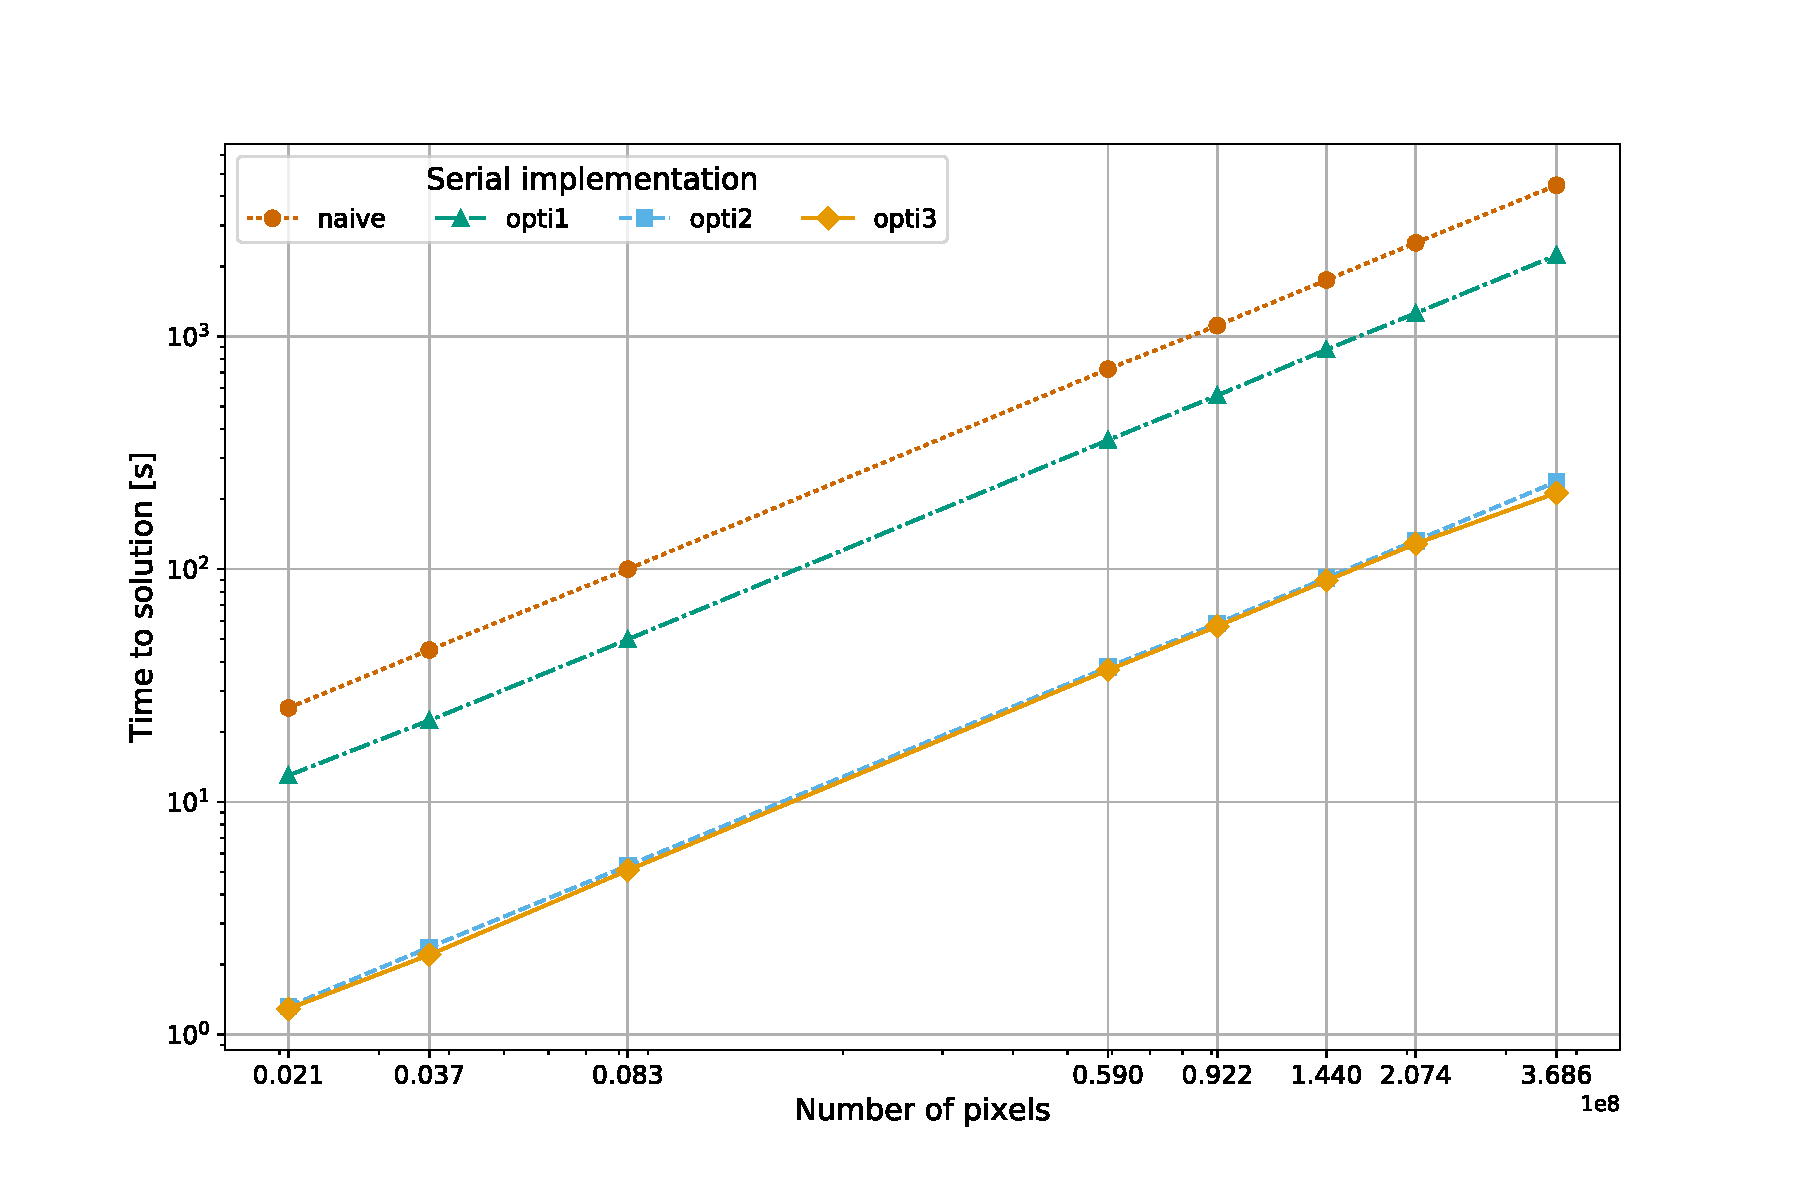
\includegraphics[width=.99\linewidth, clip, trim={1.5cm 1cm 2.5cm 2cm}]{serial-optis-px.pdf}
		\caption{} 
		\label{fig:serial-optis-px}
	\end{subfigure}%
	\begin{subfigure}{.5\textwidth}
		\centering
		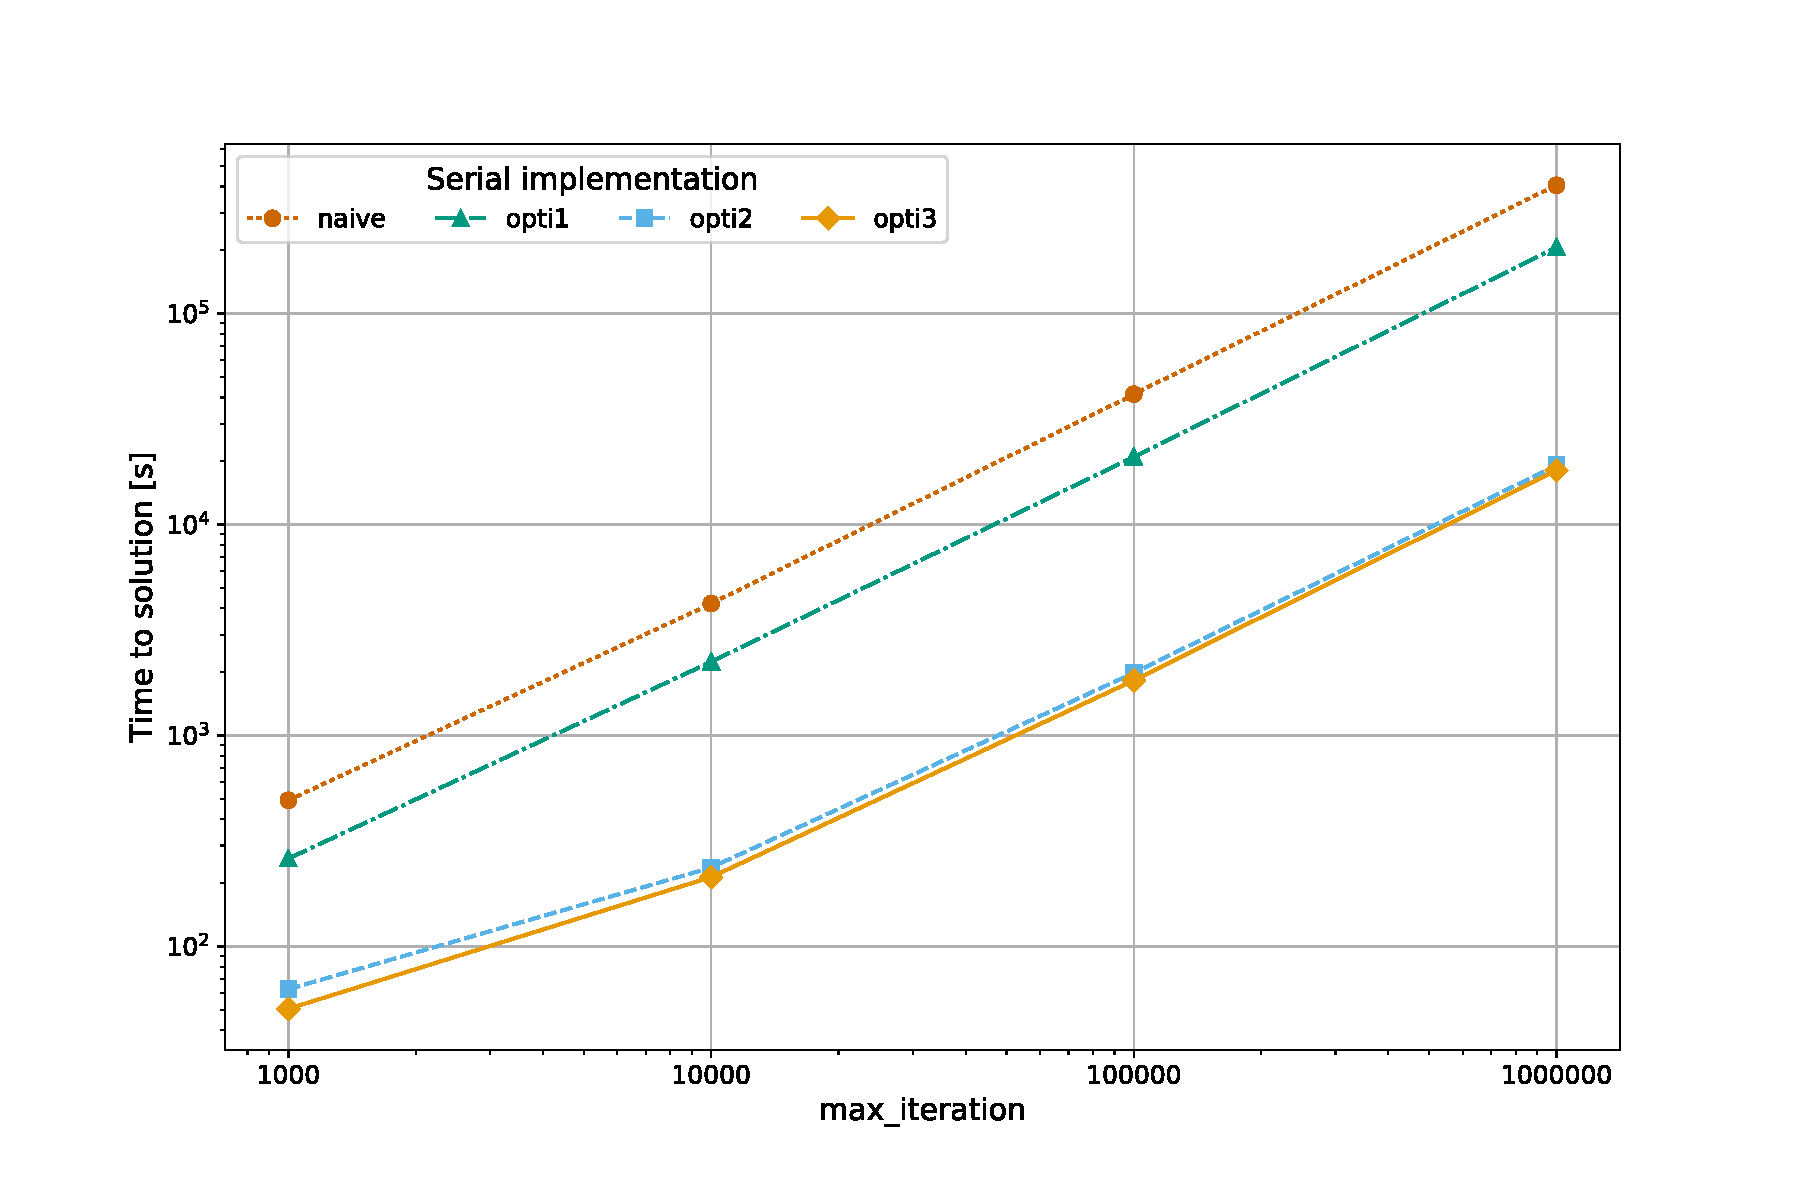
\includegraphics[width=.99\linewidth, clip, trim={1.5cm 1cm 2.5cm 2cm}]{serial-optis-maxiter.pdf}
		\caption{} 
		\label{fig:serial-optis-maxiter}
	\end{subfigure}
	\vspace{-0.4cm}
	\caption{Time to solution for the different serial implementations with respect to (a) the number of pixels (max\_iteration=10,000) and (b) max\_iteration (368,640,000 pixels).}
	\label{fig:serial-optis}
%	\vspace{-0.2cm}
\end{figure}
%\begin{figure}
%	\centering
%	\begin{subfigure}{.5\textwidth}
%		\centering
%		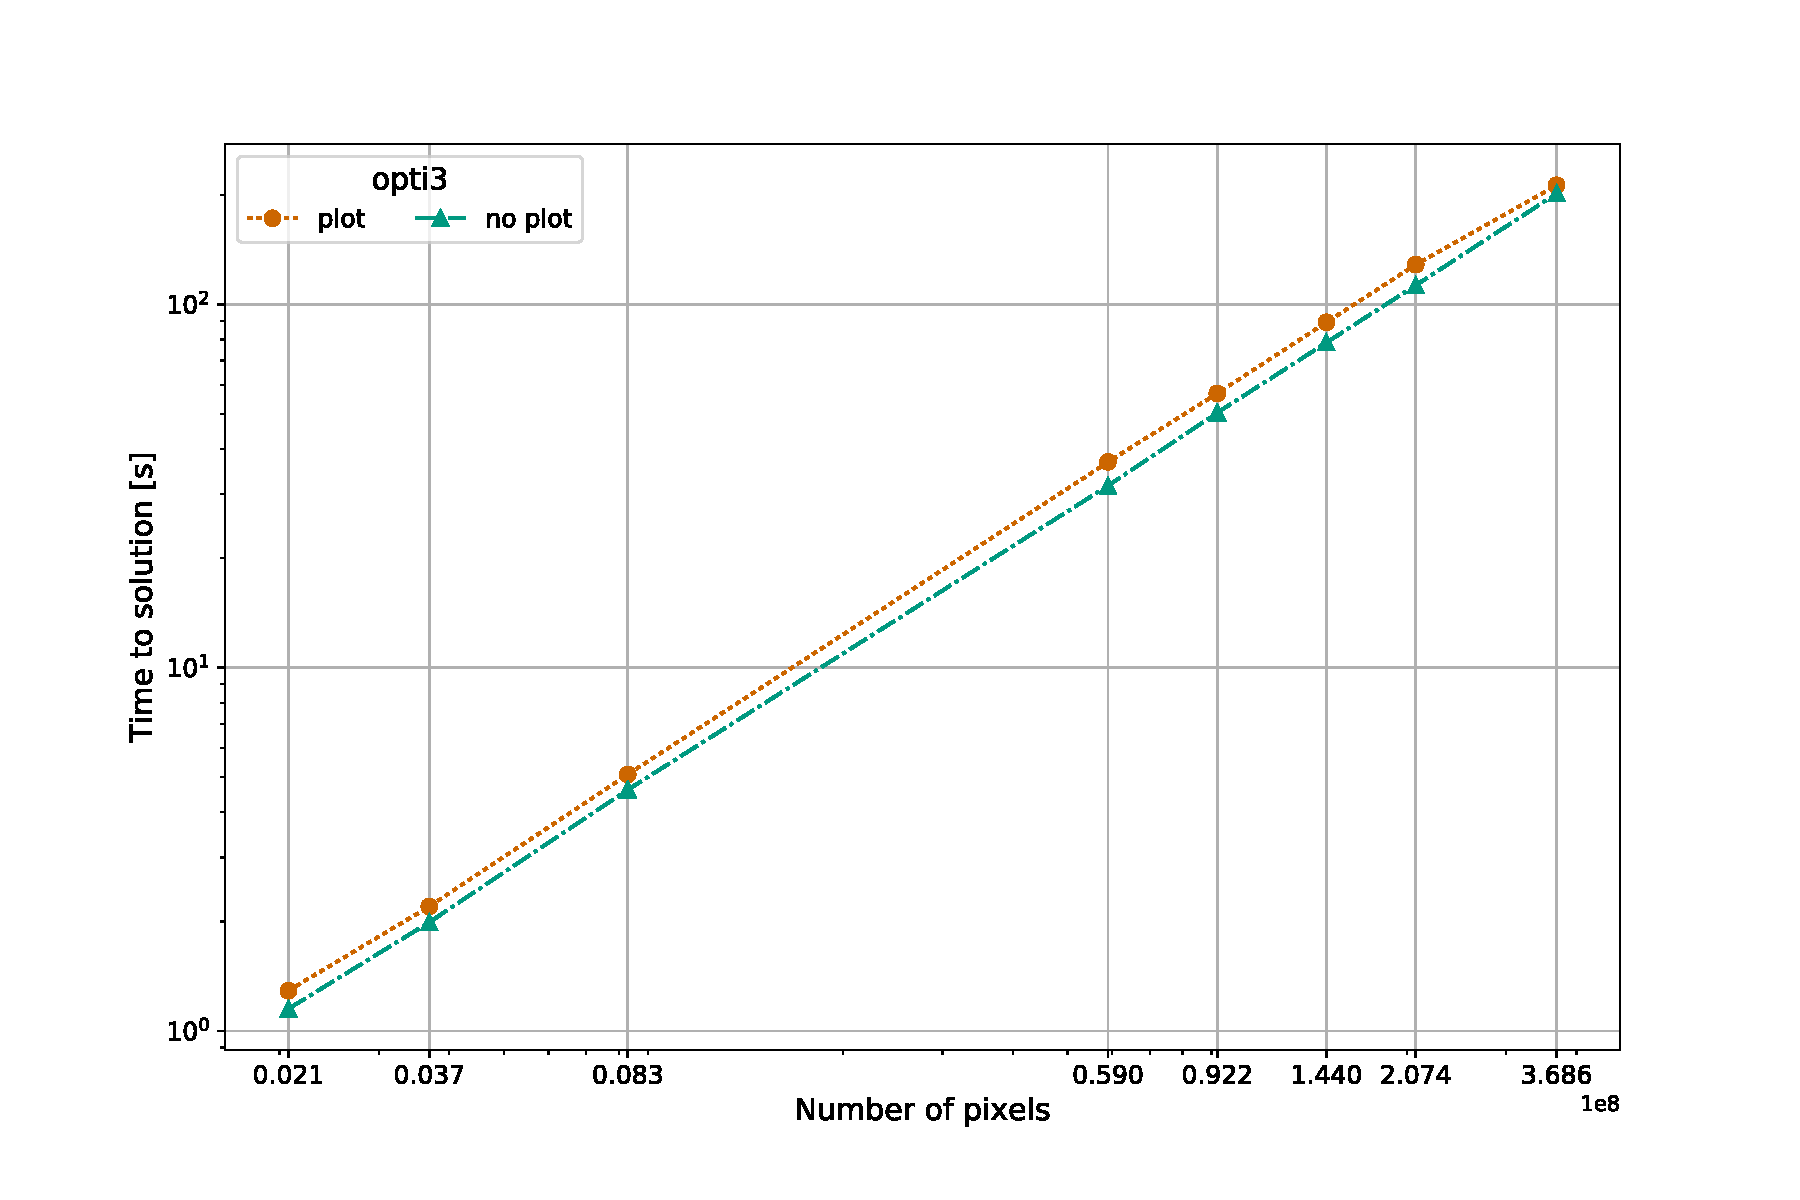
\includegraphics[width=.99\linewidth, clip, trim={1.5cm 1cm 2.5cm 2cm}]{serial-plotnoplot-px.pdf}
%		\caption{} 
%	\end{subfigure}%
%	\begin{subfigure}{.5\textwidth}
%		\centering
%		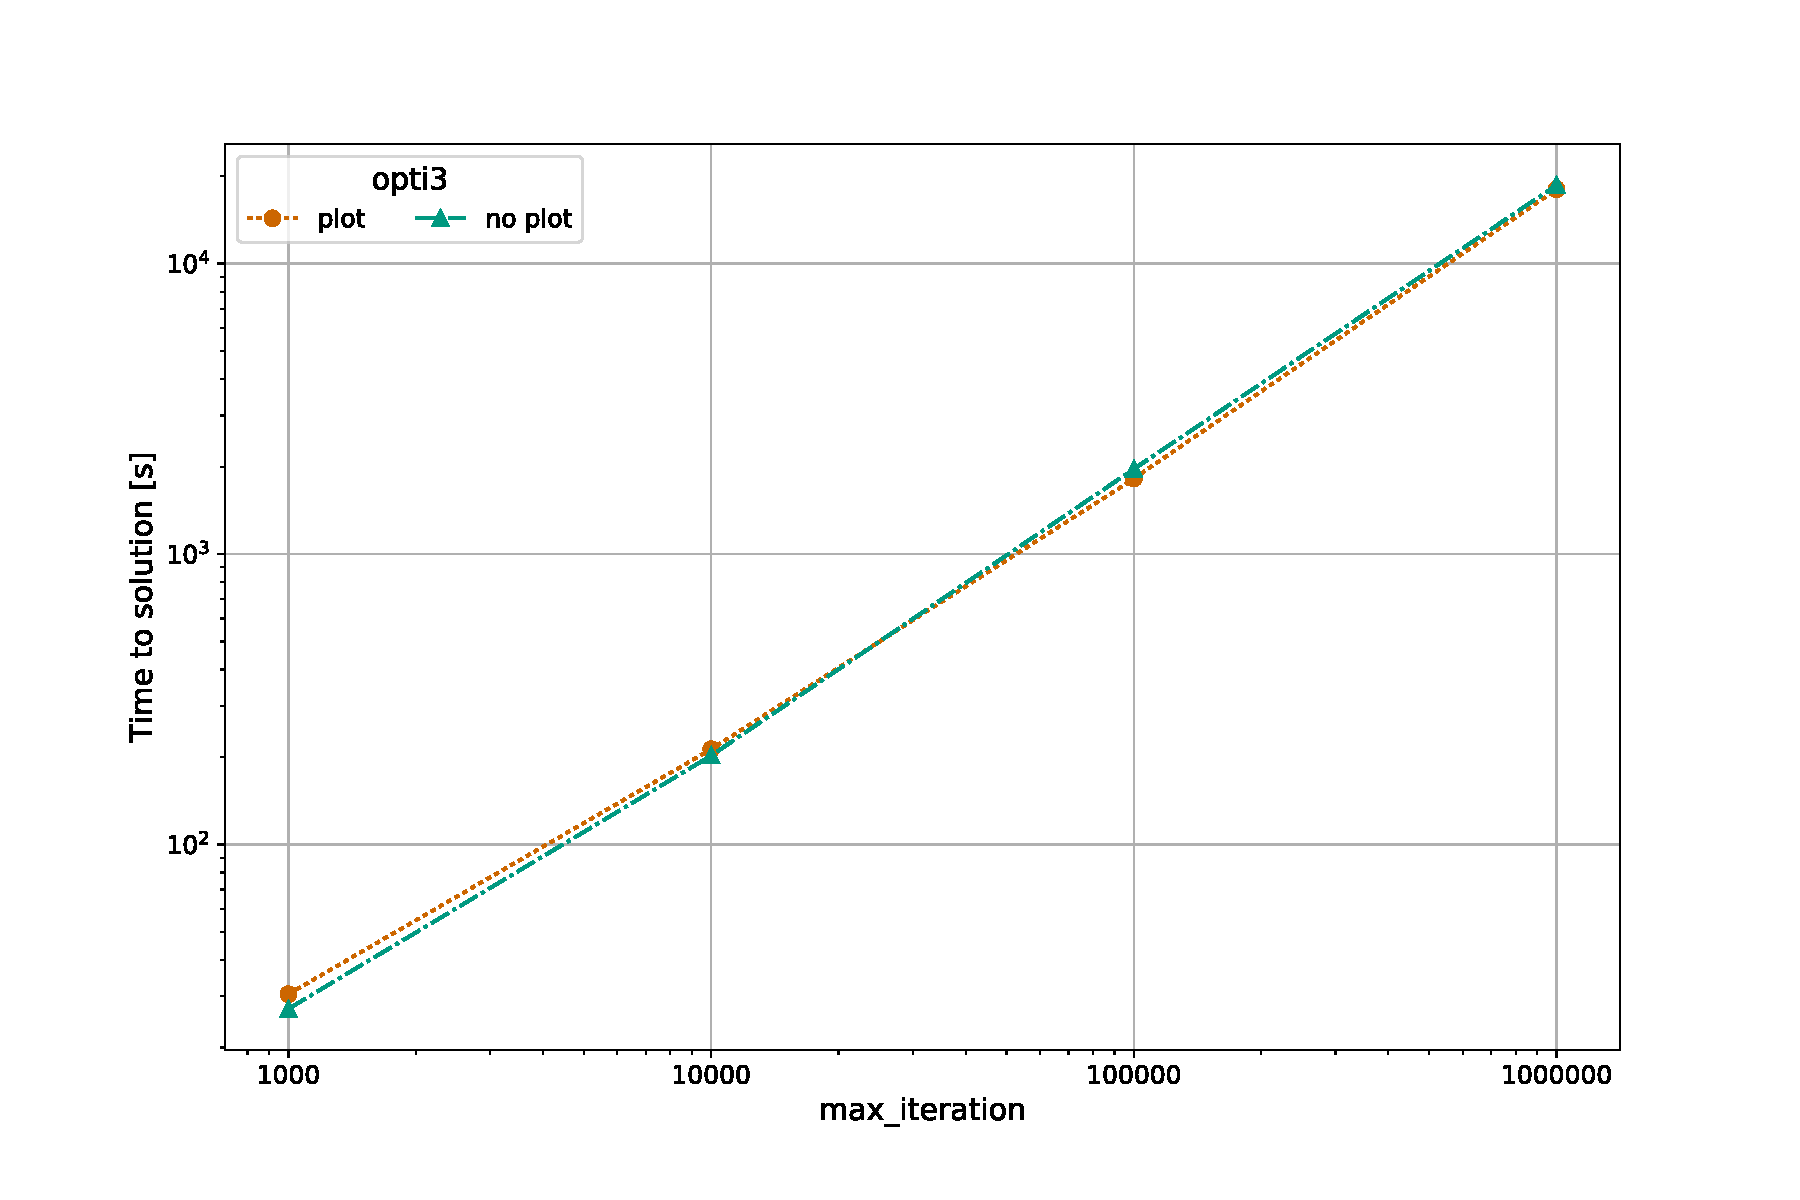
\includegraphics[width=.99\linewidth, clip, trim={1.5cm 1cm 2.5cm 2cm}]{serial-plotnoplot-maxiter.pdf}
%		\caption{} 
%	\end{subfigure}
%	\vspace{-0.4cm}
%	\caption{Time to solution of the \texttt{opti3} version when the image is plotted or not with respect to (a) the number of pixels (max\_iteration=10,000) and (b) max\_iteration (368,640,000 pixels).}
%	\label{fig:plot-noplot}
%	\vspace{-0.28cm}
%\end{figure}
\noindent
As we can see, each of these optimizations reduces the time to solution.
In particular, we halve the time to solution when we evaluate the escape time only on half image, and a drastic reduction is observed when we avoid evaluating the escape time for the sampled numbers lying within the cardioid or in the period-2 bulb as each of them would reach $max\_iteration$ otherwise.

Each of serial implementations used in generating this figure were compiled using \texttt{gcc} and setting the compiler's optimization level to \texttt{-O3} with the loop vectorizer (\texttt{-ftree-vectorize}).
In fact, this gives the best performance for each of them. 
As an example, Table \ref{tab:opti-levels} illustrates the execution times for \texttt{opti3} as it is compiled with different optimization levels.
%\begin{table}[h!]
%	\centering	
%	\vspace{-0.1cm}
%	\begin{tabular}{|l|l|} 
%		\hline
%		\textbf{Optimization level} & \textbf{Execution time [s]} \\ [0.2ex] 
%		\hline\hline
%		\texttt{-O0} & 422.91 \\ 
%		\texttt{-O1} & 230.99 \\
%		\texttt{-O2} & 208.96 \\
%		\texttt{-O3} & 208.49 \\
%		\texttt{-O3 -ftree-vectorize} & 205.41 \\ [0.2ex] 
%		\hline
%	\end{tabular}
%	\vspace{-0.1cm}
%	\caption{Execution times of \texttt{opti3} for a $25600\times14400$-pixel image and $max\_iteration=10,000$ as a function of the optimization level.}
%	\label{tab:opti-levels}
%	\vspace{-0.2cm}
%\end{table}

%Finally, Figure \ref{fig:plot-noplot} compares the times to solution of \texttt{opti3} both when the resulting image is drawn and when the execution stops just after evaluating the color of each pixel.

We also compare the times to solution of \texttt{opti3} both when the resulting image is drawn and when the execution stops just after evaluating the color of each pixel: the two curves basically overlap suggesting that the writing time is negligible.



%\subsection{Optimizations}
%
%Beside the standard sequential optimizations (loop reordering, vectorization, etc..), we put a special effort to tackle the main bottleneck of the beta-versions of the MPI and hybrid implementations : the I/O part. The current production version implements a BMP-file writer in parallel using MPI-IO. 

\vspace{-0.2cm}
\section{Prior results}

We run our implementations on the Deneb cluster at EPFL, whose specifics are~\cite{scitas}: 
\begin{itemize}
\vspace{-0.2cm}
\itemsep0em 
	
\item 376 compute nodes, each with (i) 2 Ivy Bridge processors running at 2.6 GHz, with 8 cores each, and (ii) 64 GB of DDR3 RAM.
\item 144 compute nodes, each with (i) 2 Haswell processors running at 2.5 GHz, with 12 cores each, and (ii) 64 GB of DDR4 RAM.
\item 16 GPU accelerated nodes, each with 4 K40 NVIDIA cards.
\item Infiniband QDR 2:1 connectivity.
\item GPFS filesystem.
\item Total peak performance: 293 TFLOPs (211 in CPUs, 92 in GPUs).
\end{itemize}

\vspace{-0.5cm}
\subsection{Theoretical computational cost}

In this section, we try to estimate the computational cost of the escape time algorithm.
In particular, we consider the \texttt{opti3} implementation of the algorithm.\\
For the sake of simplicity, let's consider generating square figures, where width and height have $N$ pixels.
Due to the previous symmetry optimization, the algorithm is called $N\times\frac{N}{2}$ times.\\[-8pt]

An approximation of the theoretical cost can be obtained by considering a worst-case scenario where each sampled complex number that is neither in the cardioid nor in the period-2 bulb iterates $max\_iteration$ times.\\[-7pt]

%However, we can provide a slightly better approximation by considering that the average number of iterations is independent of the number of pixels and of the maximum number of iterations, as shown in Figure \ref{fig:const}.
%\begin{figure}
%	\centering
%	\begin{subfigure}{.5\textwidth}
%		\centering
%		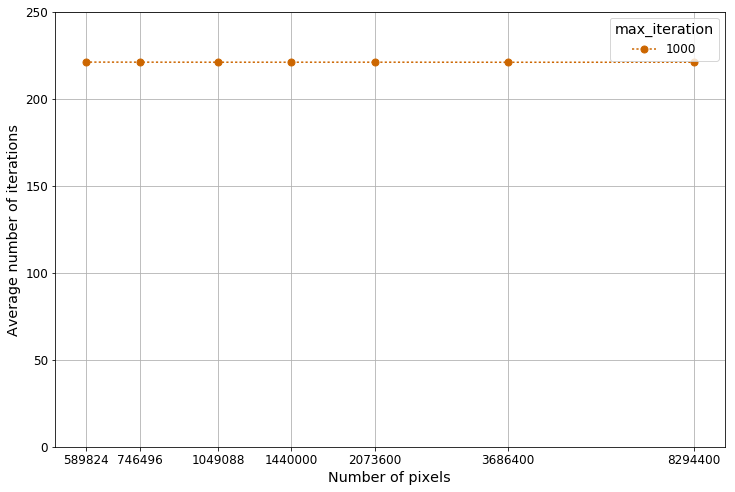
\includegraphics[width=.95\linewidth]{itersVSsize.png}
%		\caption{} 
%		\label{fig:const-size}
%	\end{subfigure}%
%	%	\begin{subfigure}{.42\textwidth}
%	%		\centering
%	%		\setlength{\figureheight}{6cm}
%	%		\setlength{\figurewidth}{6cm}
%	%		% This file was created by matplotlib2tikz v0.6.6.
\begin{tikzpicture}

\begin{axis}[
xlabel={Number of pixels},
ylabel={Average number of iterations},
xmin=516796.20197147, xmax=9466470.85821673,
ymin=0, ymax=250,
xmode=log,
width=\figurewidth,
height=\figureheight,
tick align=outside,
tick pos=left,
xmajorgrids,
x grid style={lightgray!92.026143790849673!black},
ymajorgrids,
y grid style={lightgray!92.026143790849673!black},
legend style={draw=white!80.0!black},
legend entries={{1000}},
legend cell align={left}
]
\addplot [semithick, orange!80.0!black, dotted, mark=*, mark size=3, mark options={solid}]
table {%
589824 221.155073
746496 221.118321
1049088 221.084885
1440000 221.091267
2073600 221.102072
3686400 221.059687
8294400 221.069069
};
\end{axis}

\end{tikzpicture}
%	%		\caption{Box plots for the different performance metrics.} 
%	%		\label{fig:box-plots2}
%	%	\end{subfigure}
%	\begin{subfigure}{.5\textwidth}
%		\centering
%		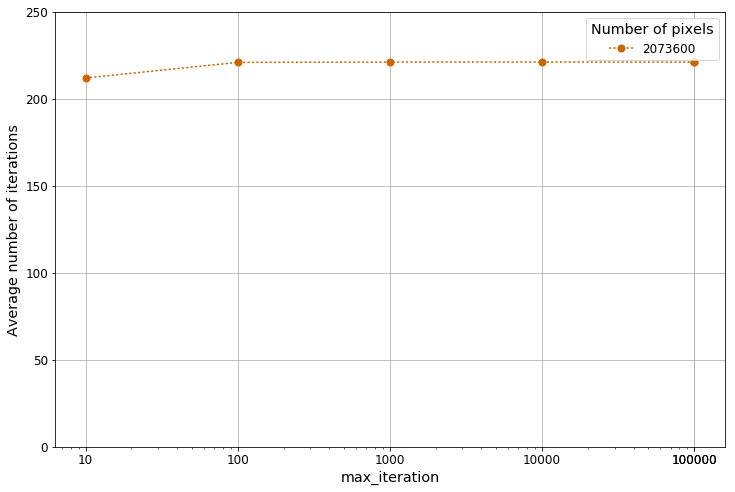
\includegraphics[width=.95\linewidth]{itersVSmaxiter.png}
%		\caption{} 
%		\label{fig:const-max}
%	\end{subfigure}
%	\caption{Evolution of the average number of iterations per pixel with respect to (a) number of pixels and (b) max\_iteration.}
%	\label{fig:const}
%\end{figure}
%Nevertheless, the execution time increases both when the number of pixels grows and when the maximum number of iterations is larger.
%This is what we expected by looking at the pictures above: most of the pixels are usually mapped to similar regions independently of the image size, and there are few pixels that iterates many times (pixels in higher-order bulbs and close to the boundaries).
%In order to obtain an optimal parallelization, we will need to properly deal with this skewness in the number of iterations (load balancing).\\
\noindent
In evaluating the computational cost, we assume the following costs per operation~\cite{costs}:
\begin{itemize}
	\vspace{-0.2cm}
	\itemsep0em 
	
	\item addition, subtraction, comparison (1);
	\item multiplication, division by 2 (4).
	\vspace{-0.15cm}
\end{itemize} 
In our implementation of the escape time algorithm, we have:
\begin{itemize}
	\vspace{-0.2cm}
	\itemsep0em 
	
	\item 5 sums, 4 multiplications and 2 divisions by 2 to initialize the variables of each pixel;
	\item 5 sums, 1 subtraction, 2 comparisons and 5 multiplications to check if the pixel is within the cardioid or in the period-2 bulb;
	\item 5 sums, 1 subtraction, 2 comparisons and 3 multiplications in each iteration.
\end{itemize}
\vspace*{-1.1cm}
Note that these are simple approximations and the real cost of each operation actually depends on the computer architecture.
Furthermore, we are ignoring the cost of conditional statements which lead to expensive branch mispredictions.\\
That said, an estimation of the computational cost for an $N\times N$-pixel image is then given by:
\vspace{-0.15cm}
$$\approx (c + 0.76\times max\_iteration) \times \dfrac{N^2}{2}$$
\vspace{-0.1cm}
%\begin{multline*}
%\frac{N^2}{2}\times[\left(5\times1 + 4\times4 + 2\times4\right) + \\
%\left(5\times1 + 1\times1 + 2\times1 + 5\times4\right) + \\
%\left(1-0.34\right)\times221\times\left(5\times1 + 1\times1 + 2\times1 + 3\times4\right)]
%\end{multline*}
%\begin{multline*}
%\approx c\times N^2~~~~~~~~~~~~~~~~~~~~~~~~~~~~~~~~~~~~~~~~~~~~~~~~~~~~~~~~~~~~~~~~~~~~~~~~~~~~~~~~~~~~~~~~~~~~~~~~~~~~~~~~~~~~~~~~~~~~~~~~~~~~~~~~~~~~~~~~~~
%\end{multline*}
\noindent
Where $0.76$ is the percentage of pixels that are neither in the cardioid nor in the period-2 bulb and $c\approx 57$.
Hence, the algorithm's computational cost is $O(N^2)$ and so linear in the number of pixels (as we expected from its formulation).\\[-7pt]

Note that this cost does not take into account the expensive operation to determine the smooth color for each pixel and the additive time needed to store the matrix of iterations as an image, which are also $O(N^2)$.
Memory requirements are in the order of $O(N^2)$ too.\\[-7pt]

Finally, if we fix the size of the image, then the computational time increases linearly with the value of $max\_iteration$.
All these relationships are confirmed by the curves in Figure \ref{fig:serial-optis}.

\vspace{-0.1cm}
\subsection{Strong scaling}
Strong scaling means using parallel computing to run a problem faster than on a single core.\\
Strong scaling is usually equated with Amdahl's Law, which specifies the maximum speedup that can be expected by parallelizing portions of a serial program:
\vspace{-0.1cm}
$$S_p = \frac{1}{\alpha + \frac{1 - \alpha}{p}} = \frac{T_1}{T_p}$$
Where $\alpha$ is the fraction of non-parallelizable code, $p$ is the number of processors, and $T_1$ and $T_p$ are the execution times on one and p processors, respectively.\\[-7pt]

Hence, we need to estimate the fraction of non-parallelizable code $\alpha$.
The core of the algorithm is intrinsically parallel because of the independence of the computations between the pixels.
However, serial sequences are present as well to (i) allocate and deallocate the variables, (ii) set the corresponding number of iterations in the other half of the image and (iii) store the resulting image onto disk.
The impact of the serial part will be more and more evident as the size of the image (number of pixels) increases.\\
We use \texttt{gprof} to obtain an estimation of the value of $\alpha$.
In particular, we do this when drawing both a 4K image ($8,294,400$ pixels) and a $25600\times14400$ image ($368,640,000$ pixels).
In both cases we set $max\_iteration$ to $10,000$.
The value of $\alpha$ is estimated to be $0$ in the former case, while equal to $1.91$ in the latter; hence suggesting a perfect speedup for relatively small images.\\
Figure \ref{fig:exp-speedup} shows the expected speedup in these two scenarios.
\begin{figure}[H]
	\centering
	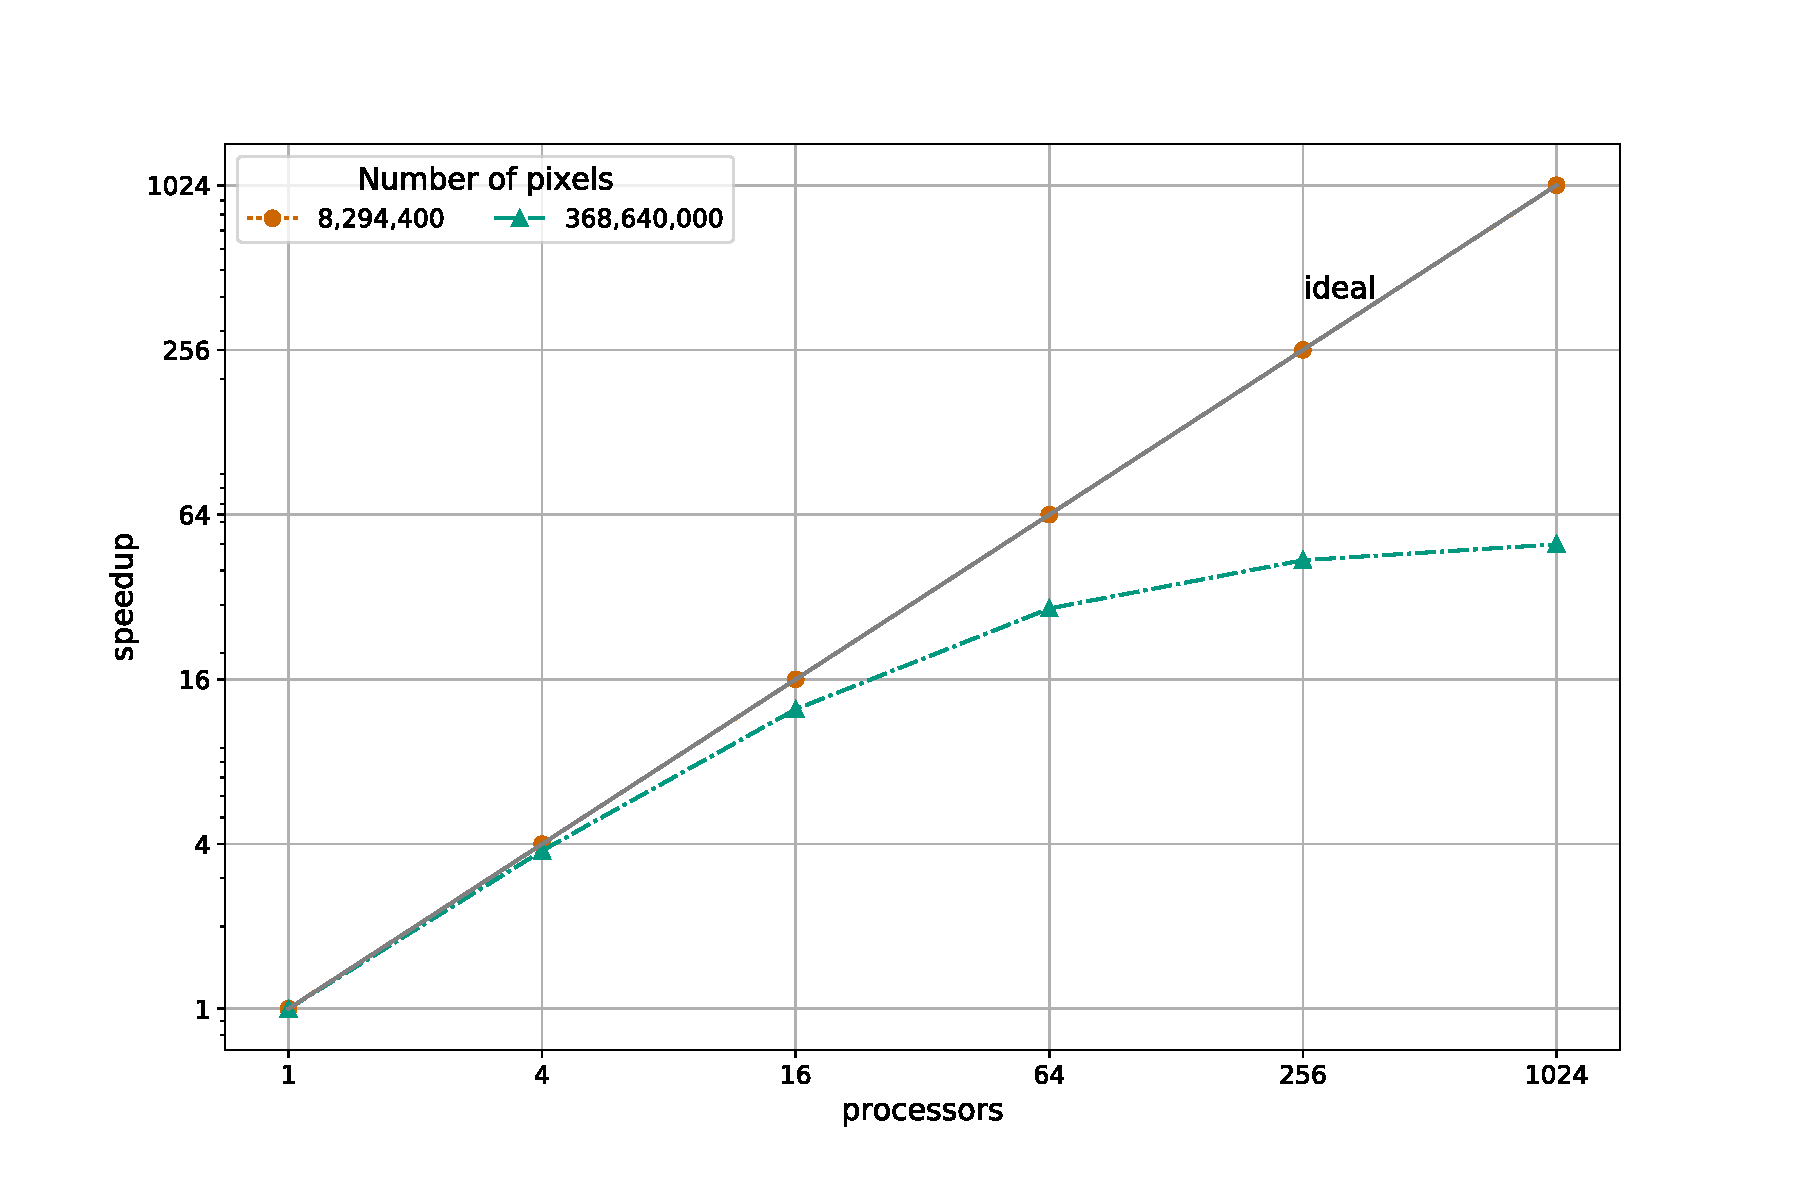
\includegraphics[width = 0.5\textwidth, clip, trim={1.5cm 1cm 2cm 2cm}]{expected-speedup.pdf}
	\caption{Expected speedup for small ($\alpha=0\%$) and large ($\alpha=1.91\%$) images from Amdahl's law.}
	\label{fig:exp-speedup}
\end{figure}

%\begin{figure}[ht]
%	\centering
%	\setlength\figureheight{10cm}
%	\setlength\figurewidth{16cm}
%	% This file was created by matplotlib2tikz v0.6.6.
\begin{tikzpicture}

\definecolor{color0}{rgb}{0,0.6,0.5}
\definecolor{color1}{rgb}{0,0.6,0.498039215686275}

\begin{axis}[
xlabel={processors},
ylabel={speedup},
xmin=0.707106781186548, xmax=1448.15468787005,
ymin=0.707106781186548, ymax=1448.15468787005,
xmode=log,
ymode=log,
width=\figurewidth,
height=\figureheight,
tick align=outside,
tick pos=left,
xmajorgrids,
x grid style={lightgray!92.026143790849673!black},
ymajorgrids,
y grid style={lightgray!92.026143790849673!black},
legend cell align={left},
legend style={at={(0.03,0.97)}, anchor=north west, draw=white!80.0!black},
legend entries={{8,294,400},{368,640,000}}
]
\addplot [semithick, orange!80.0!black, dotted, mark=*, mark size=3, mark options={solid}]
table {%
1 1
4 4
16 16
64 64
256 256
1024 1024
};
\addplot [semithick, color0, dash pattern=on 1pt off 3pt on 3pt off 3pt, mark=triangle*, mark size=3, mark options={solid,fill=color1}]
table {%
1 1
4 3.7832214130332
16 12.4368441507967
64 29.0473380837834
256 43.6078698577634
1024 49.8556425973621
};
\addplot [semithick, gray]
table {%
1 1
4 4
16 16
64 64
256 256
1024 1024
};
\node at (axis cs:257,396)[
  scale=0.72,
  anchor=base west,
  text=black,
  rotate=0.0
]{ ideal};
\end{axis}

\end{tikzpicture}
%	\caption{Box plots for the different performance metrics.} 
%	\label{fig:exp-speedup}
%\end{figure}


\subsection{Weak scaling}
Weak scaling is what we refer to when we are talking about using parallel computing to run a larger problem in the same amount of time as a smaller one on a single core.
In other words, it is a measure of how the time to solution changes as more processors are added to a system with a fixed problem size per processor.\\[-7pt]
%Weak scaling is often equated with Gustafson's Law, which states that the problem size scales with the number of processors:
%$$S_p = p - \beta(n)\left(p - 1\right) = \frac{T_1}{T_p}$$
%Where $\beta$ is the fraction of non-parallelizable code and $n$ is the problem size.\\

We expect a significant speedup also in this case, but we are somehow limited by the size of the images we can create.
So, we can instead increase the complexity of the problem by choosing larger values of $max\_iteration$.
Knowing that the peak number of floating-point operations per second in one TESLA K40 GPU card is $1.43~TFLOPs$ for double-precision and $4.29~TFLOPs$ for single-precision~\cite{gpus}, while having a peak of $\frac{211}{376\times2\times8 + 144\times2\times12}\approx22.3~GFLOPs$ in a single core of CPU in the Deneb cluster, we can predict solving problems that are $\approx66$ (double-precision) or $\approx197$ (single-precision) times larger on the GPU in the same time as a reference problem on a single CPU core.
Despite this wide gap, we should remember that these are theoretical predictions and several issues will actually limit the parallel performance, such as memory communication overheads and load balancing.

\vspace{-0.2cm}
\section{Going parallel}

After having debugged, profiled and optimized our serial code, we can proceed with the parallelization phase.
In fact, since each element in the array is independent of all the others, our algorithm leads to an embarrassingly parallel formulation.

\vspace{-0.2cm}
\subsection{CUDA implementations}

We start parallelizing our code with CUDA; once this version is optimized, we will add MPI.\\[-7pt]

Firstly, we just port \texttt{opti3} to CUDA. 
We do so by parallelizing the core of the algorithm: that is, evaluating the escape times for each of the points in the bottom half of the figure.
This version is still far from optimal: most of the time spent by the serial code is in computing the color associated to a given iteration value and this part is still done serially.
Moreover, we still use three matrices: one for the escape times, one for the real parts reached by the quadratic mappings and one for the corresponding imaginary parts.
Sending three matrices on the PCIe bus surely does not lead to high performance computing, but this version serves as a first working CUDA implementation of the algorithm.\\[-7pt]

After debugging this version, we proceed implementing a new one: \texttt{opti4}.
In this version, all the workload is carried out by the GPU.
The only values exchanged by the between CPU and the GPU are the chars representing the RGB values for each pixel in the bottom half of the image.
The code is split into serial part (\texttt{.c}) and parallel part (\texttt{.cu}), compiled with \texttt{gcc} and \texttt{nvcc}, respectively, and then linked together into one executable.
To do so, we need a C wrapper for the kernel that allows the CPU to share parameters with the CUDA part.
Moreover, all the constant values are copied to the Constant memory: a read-only, quick cache that can broadcast to all active threads.\\
When we profile this application with \texttt{nvprof}, we notice that it is compute-bound: that is, its arithmetic intensity is underneath the peak performance ceiling in the Roofline model.\\[-7pt]

Finally, we move from a double-precision to a single-precision representation with \texttt{opti5}.
Strictly speaking, the resulting drawings are different from the previous ones but no human being would be able to tell the difference between two images produced using double-precision and single-precision operands.
We make this shift to single precision in order to maximize instruction throughput (as we described above and it is suggested in \cite{guide}).\\
The resulting optimization is still compute-bound.\\[-7pt]

\noindent
The performances of the presented CUDA optimizations are compared in Figure \ref{fig:cuda-optis}.\\[-7pt]
\begin{figure}[t]
	\vspace{-0.7cm}
	\centering
	\begin{subfigure}{.5\textwidth}
		\centering
		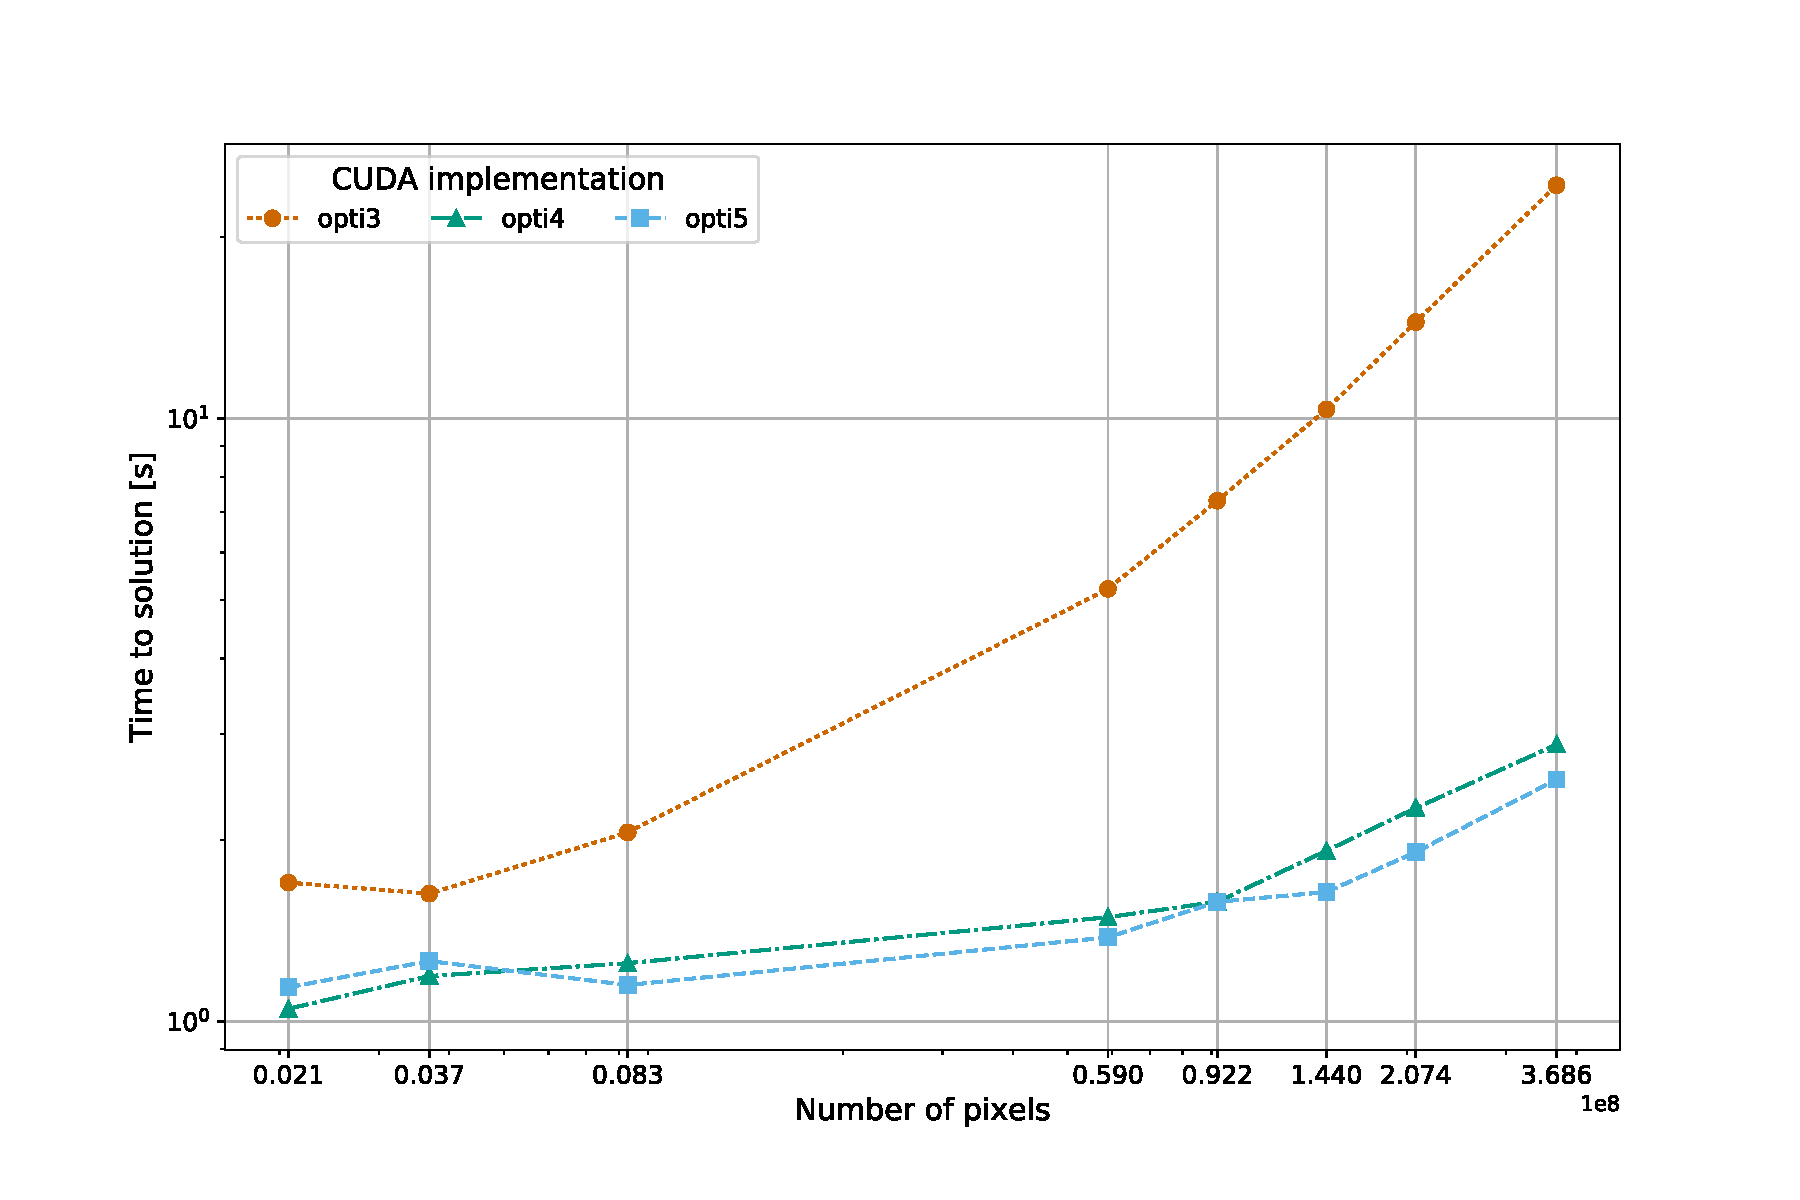
\includegraphics[width=.99\linewidth, clip, trim={1.5cm 1cm 2.5cm 2cm}]{cuda-optis-px.pdf}
		\caption{} 
		\label{fig:cuda-optis-px}
	\end{subfigure}%
	\begin{subfigure}{.5\textwidth}
		\centering
		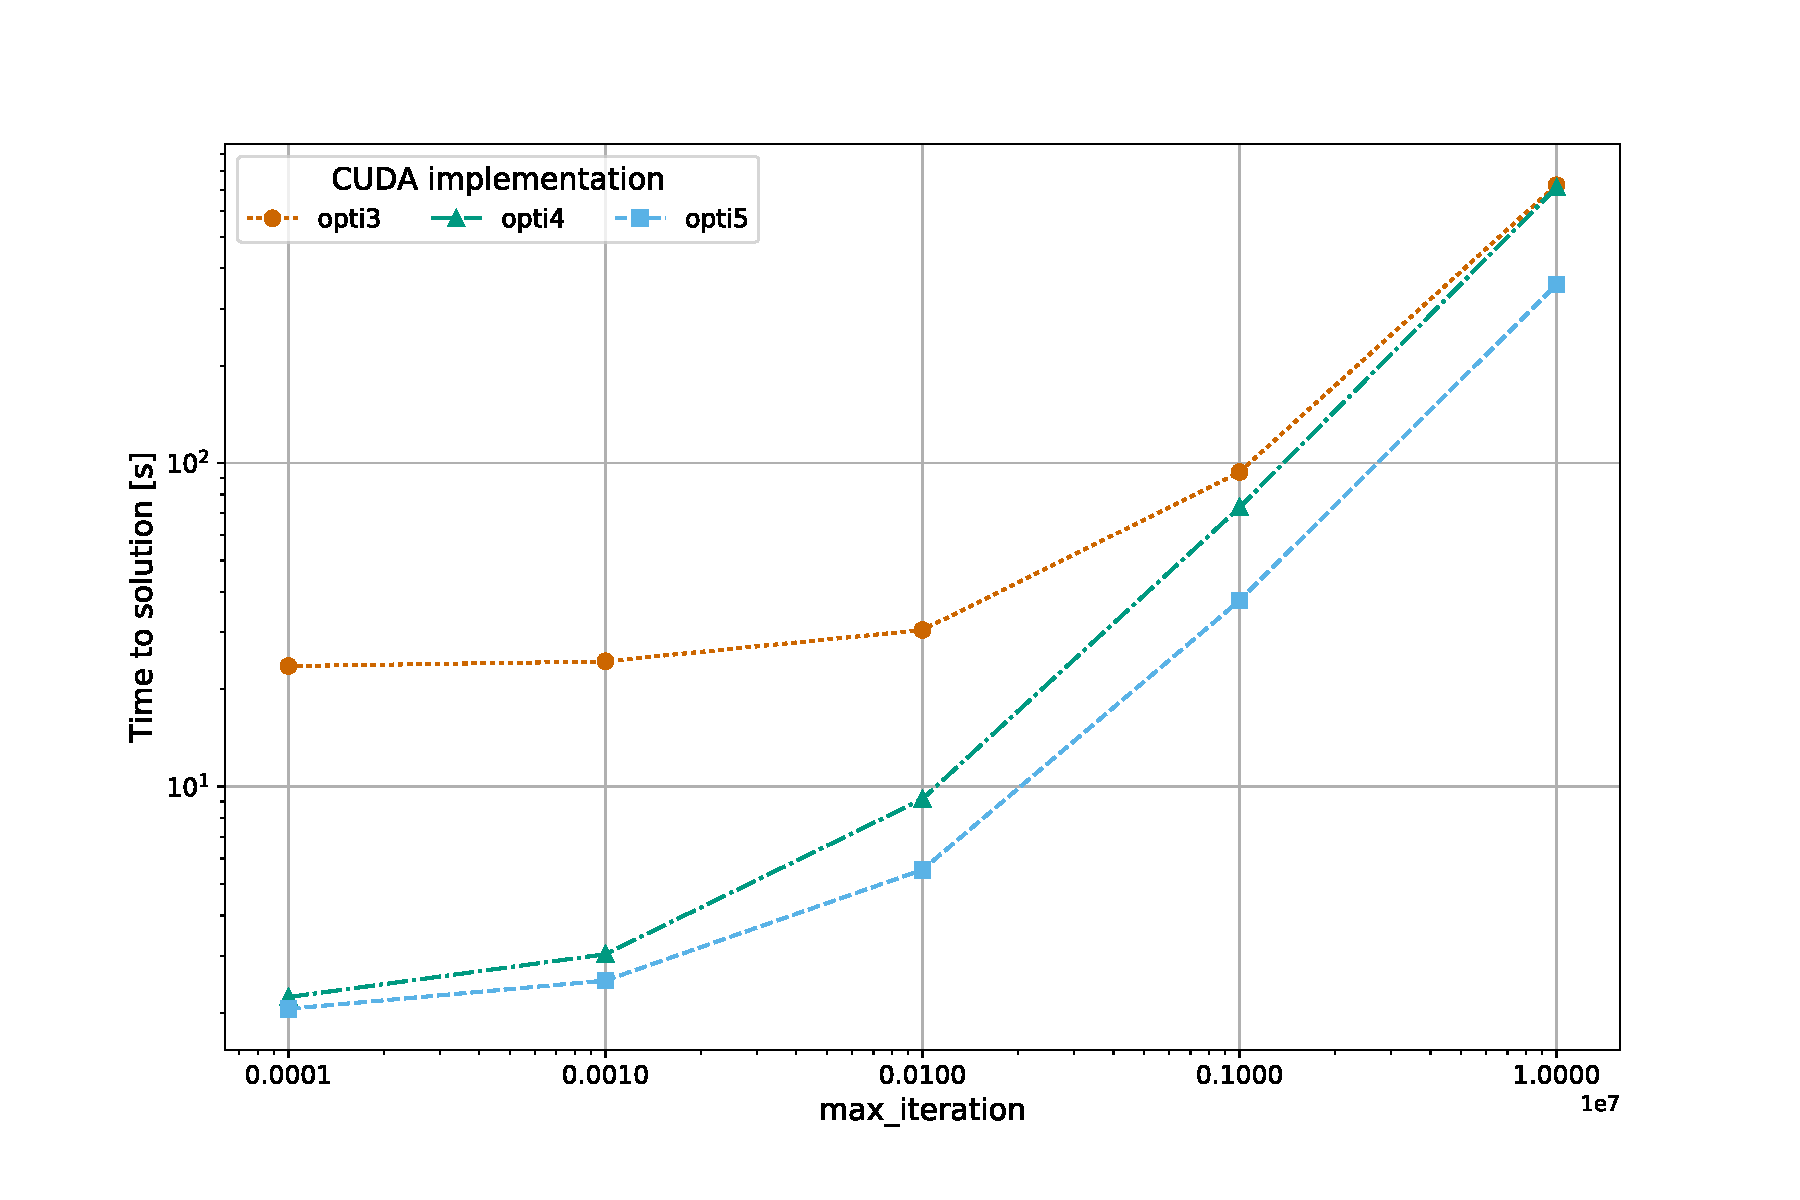
\includegraphics[width=.99\linewidth, clip, trim={1.5cm 1cm 2.5cm 2cm}]{cuda-optis-maxiter.pdf}
		\caption{} 
		\label{fig:cuda-optis-maxiter}
	\end{subfigure}
	\vspace{-0.4cm}
	\caption{Time to solution for the CUDA implementations with respect to (a) the number of pixels (max\_iteration=10,000) and (b) max\_iteration (368,640,000 pixels) with block size $512\times1$.}
	\label{fig:cuda-optis}
\vspace{0.3cm}
\end{figure}

We complete our study on CUDA by tuning the \textit{block size} used by \texttt{opti5}.
This is a crucial hyperparameter that leads to performance improvements and it is determined by both the problem at hand and the specifics of the used GPU.
A properly set block size leads to increased occupancy; i.e., the ratio between the number of active warps per multiprocessor and the maximum number of active warps.
Table \ref{tab:block-size} presents the achieved occupancy as a function of the block size for two image sizes when launched on Deneb.
The winning size is \texttt{256$\times$1}.
We make use of \texttt{nvprof} to evaluate the occupancy.
Even though larger image sizes and higher $max\_iteration$ would lead to a more accurate evaluation of the achieved occupancy, we had to set $max\_iteration$ to only $10,000$ in order for \texttt{nvprof} to evaluate this metrics.
Nevertheless, the highest achieved occupancy is close to $66\%$, which is enough to usually saturate the bandwidth~\cite{occupancy}.
Further, one should look at increasing occupancy only if the the kernel is bandwidth-bound, which is not our case.
\begin{table}[H]
	\begin{subtable}{.5\linewidth}
		\centering
		\begin{tabular}{|l|l|l|} 
			\hline
			\textbf{Block size} & \multicolumn{2}{|c|}{\textbf{Occupancy [$\%$]}} \\
			\cline{2-3}
			 & \texttt{2560x1440} & \texttt{25600x14400} \\ [0.2ex] 
			\hline\hline
			\texttt{32x1} & 18.05 & 18.81 \\ 
			\texttt{64x1} & 25.41 & 32.65 \\
			\texttt{128x1} & 31.82 & 51.52 \\
			\texttt{192x1} & 34.85 & 56.01 \\
			\texttt{256x1} & \textbf{36.15} & \textbf{58.80} \\
			\texttt{384x1} & 35.62 & 57.30 \\
			\texttt{512x1} & 28.76 & 52.37 \\
%			\texttt{768x1} & 13.79 & 37.59 \\
			\texttt{1024x1} & 8.39 & 25.50 \\
			\texttt{8x8} & 19.04 & 20.12 \\
			\texttt{16x16} & 26.91 & 25.93 \\
			\texttt{32x32} & 5.91 & 7.74 \\ [0.2ex] 
			\hline
		\end{tabular}
		\caption{}
	\end{subtable}%
	\begin{subtable}{.5\linewidth}
		\centering
		\begin{tabular}{|l|l|l|} 
			\hline
			\textbf{Block size} & \multicolumn{2}{|c|}{\textbf{Execution time [s]}} \\
			\cline{2-3}
			& \texttt{2560x1440} & \texttt{25600x14400} \\ [0.2ex] 
			\hline\hline
			\texttt{32x1} & 2.53 & 79.61 \\ 
			\texttt{64x1} & 2.29 & 50.32 \\
			\texttt{128x1} & 2.10 & 37.52 \\
			\texttt{192x1} & 2.05 & 36.56 \\
			\texttt{256x1} & \textbf{2.04} & \textbf{35.91} \\
			\texttt{384x1} & 2.11 & 36.60 \\
			\texttt{512x1} & 2.17 & 37.69 \\
%			\texttt{768x1} & 2.38 & 44.73 \\
			\texttt{1024x1} & 5.65 & 90.60 \\
			\texttt{8x8} & 4.09 & 237.72 \\
			\texttt{16x16} & 2.45 & 97.12 \\
			\texttt{32x32} & 7.48 & 270.24 \\ [0.2ex] 
			\hline
		\end{tabular}
		\caption{}
	\end{subtable} 
	\caption{(a) Occupancy and (b) execution time for two image sizes as the block size varies.}
	\label{tab:block-size}
\end{table}


\vspace*{-0.27cm}
\subsection{Hybrid implementations}

After having optimized on a single GPU, we introduce an additional layer of parallelization: we distribute the computations over different CPUs and GPUs with MPI.
Specifically, we split the bottom half of the image to all the reserved GPUs by rows, and so each GPU receives the same number of pixels~\footnote{If dividing the number of rows by the number of GPUs does not return an integer, the remaining rows are assigned as uniformly as possible among all the GPUs.}.\\
Each GPU node on Deneb has two processors and four GPUs.
We then distribute \texttt{opti5} so as to make use of the resources available on a single node; we do so with two versions.\\[-7pt]

Firstly, we distribute the image to the two processors and each of them uses one GPU to evaluate the escape times and the corresponding colors.
We provide two implementations: a first implementation using non-blocking, point-to-point communications where the processor with rank $0$ receives the image parts in an out-of-order fashion.
In particular, no \texttt{MPI\_Barrier()} is used.
The second implementation, instead, makes use of parallel I/O to increase the writing performance on the GPFS parallel file system.\\[-7pt]

Secondly, we distribute the image to the two processors and each of them uses two GPUs.
That is, each processor is in charge of half of the bottom half image, which is then further split to the two GPUs.
In this scenario, to achieve the highest performance, all the CUDA functions are asynchronous (with no barrier or thread synchronization used).
Also this version comes with both the centralized, non-blocking implementation and the one using parallel I/O.\\[-7pt]

The performances of the hybrid implementations are shown in Figure \ref{fig:hybrid-optis}, where we can see that the benefits of using multiple GPUs is manifested only for massive loads.
\begin{figure}
	\vspace{-0.7cm}
	\centering
	\begin{subfigure}{.5\textwidth}
		\centering
		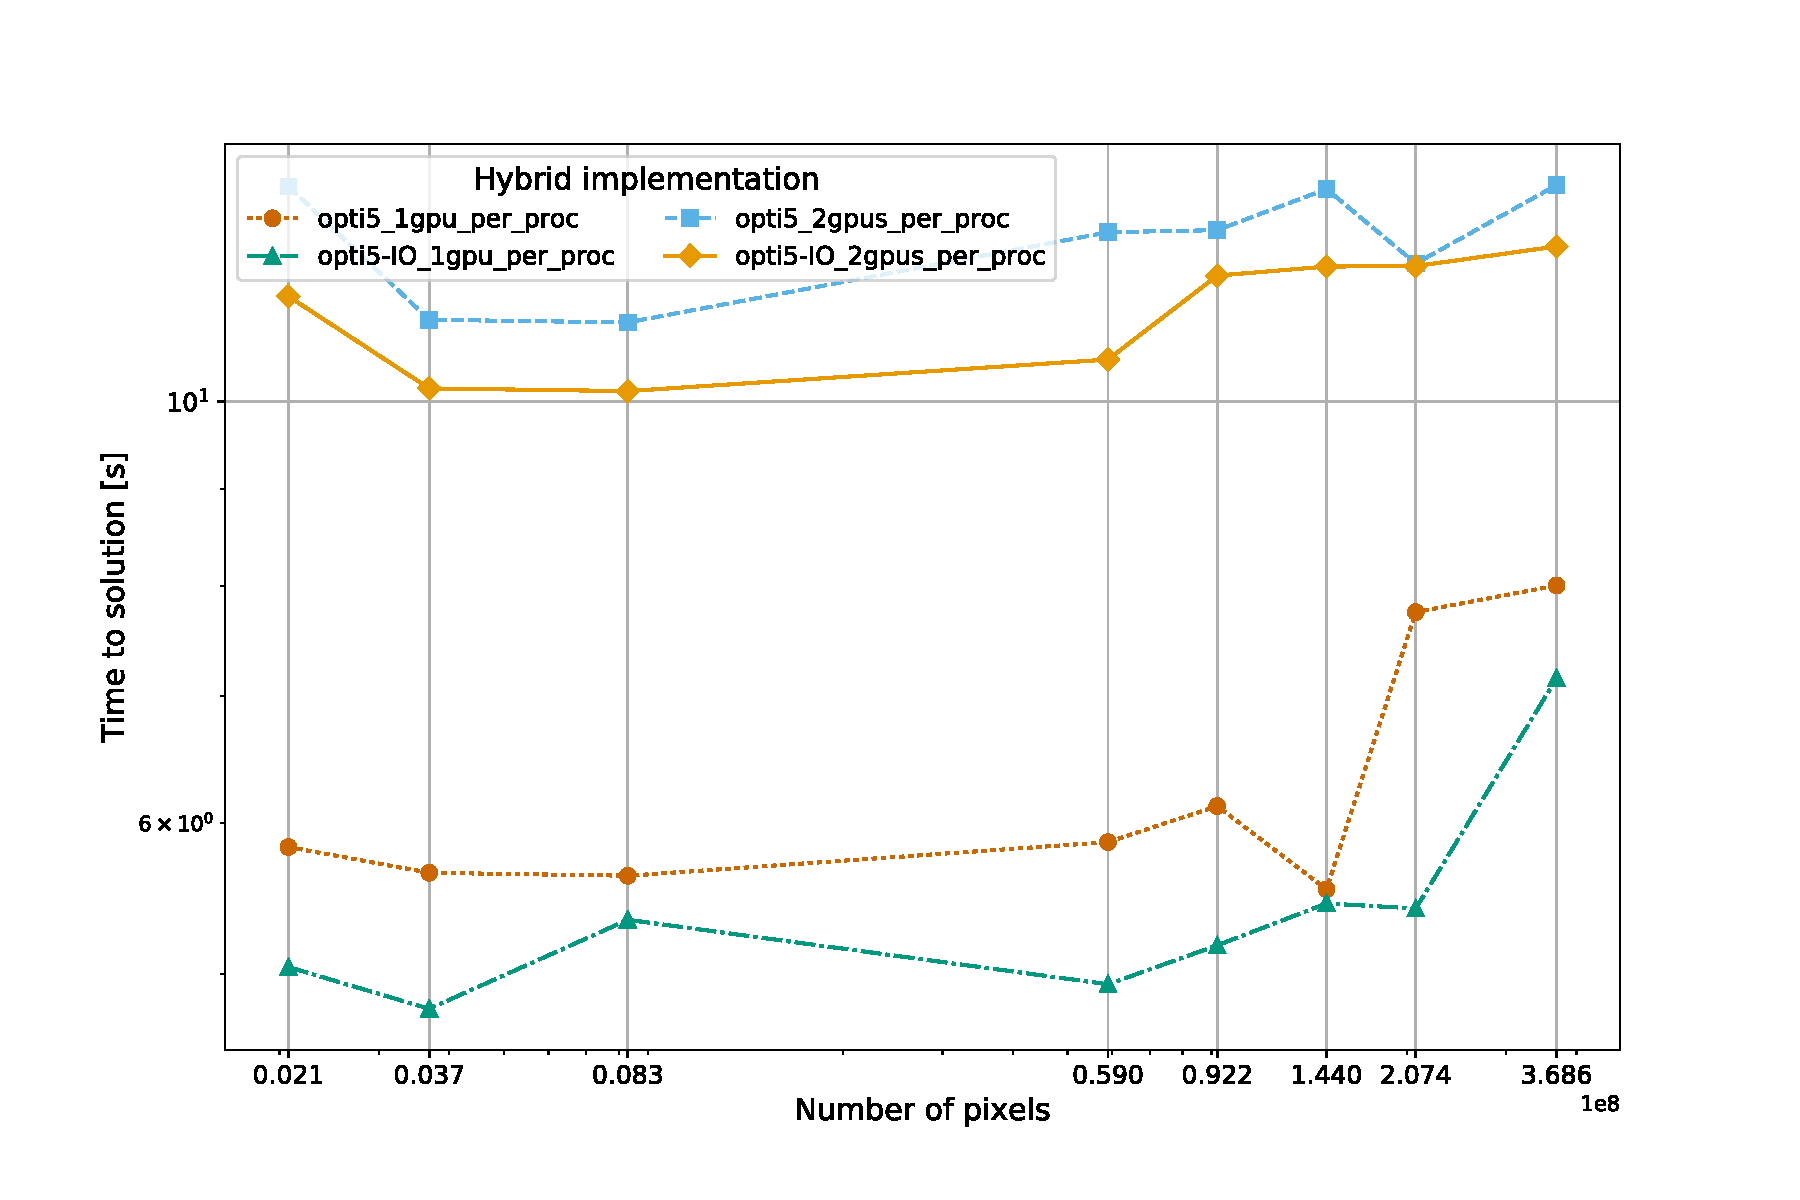
\includegraphics[width=.99\linewidth, clip, trim={1.5cm 1cm 2.5cm 2cm}]{hybrid-optis-px.pdf}
		\caption{} 
		\label{fig:hybrid-optis-px}
	\end{subfigure}%
	\begin{subfigure}{.5\textwidth}
		\centering
		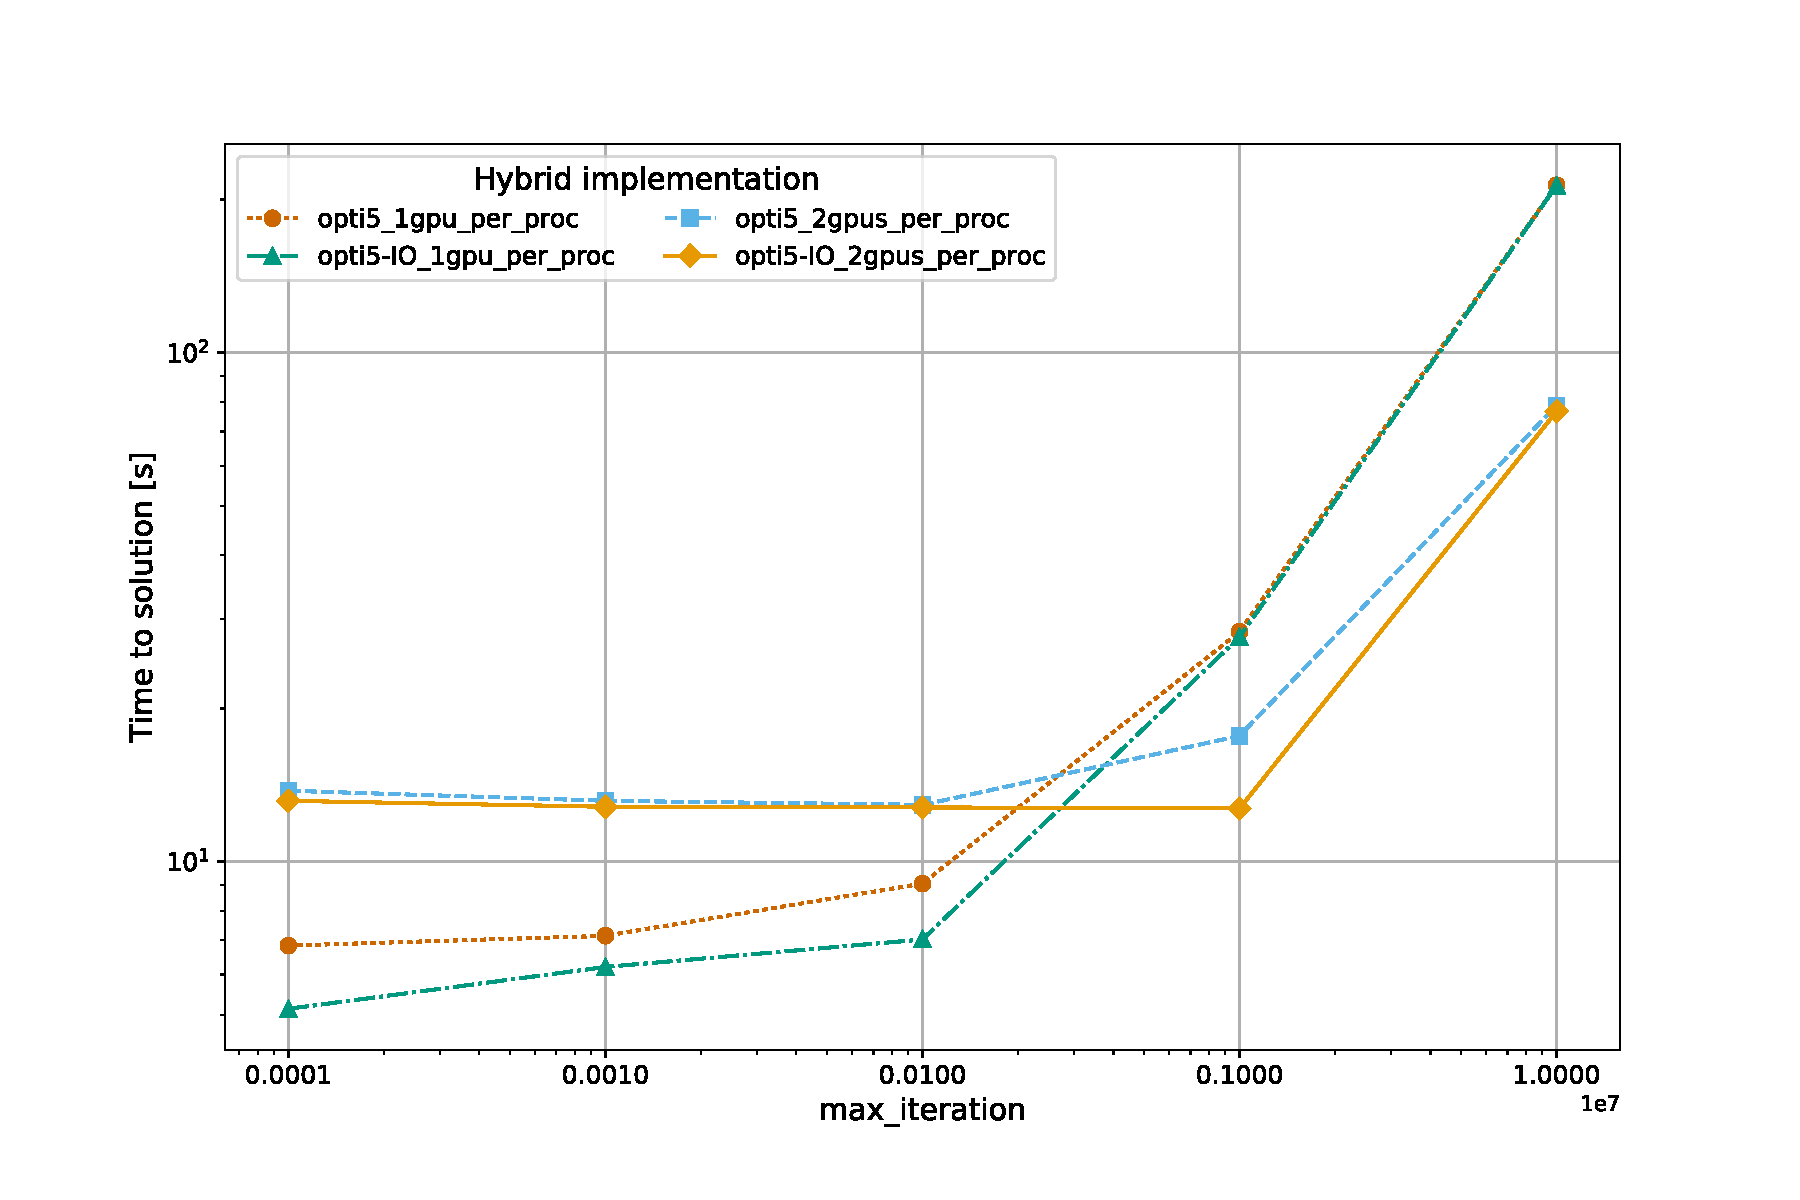
\includegraphics[width=.99\linewidth, clip, trim={1.5cm 1cm 2.5cm 2cm}]{hybrid-optis-maxiter.pdf}
		\caption{} 
		\label{fig:hybrid-optis-maxiter}
	\end{subfigure}
	\vspace{-0.4cm}
	\caption{Time to solution for the hybrid implementations with respect to (a) the number of pixels (max\_iteration=10,000) and (b) max\_iteration (368,640,000 pixels) with block size $256\times1$.}
	\label{fig:hybrid-optis}

\end{figure}


\vspace{-0.2cm}
\section{Final results}

In this section, we present the results we obtained for scaling when CUDA and MPI are used.\\
The results using multiple GPUs versions are obtained from the parallel I/O implementations.\\[-7pt]

Figure \ref{fig:strong} presents the results for strong scaling: specifically, for a $25600\times14000$-pixel image and $max\_iteration=10,000,000$.\\
Figure \ref{fig:strong-mpi} shows how increasing the number of GPUs affects the speedup: here, we can see that the speedup obtained using four GPUs is higher than the ideal one.
This can be explained by the fact that all the CUDA functions are called asynchronously in this version and both the multi-GPU versions use two processors.\\
Figure \ref{fig:strong-tts} illustrates how the time to solution varies from the serial version to the hybrid version.\\[-7pt]
\begin{figure}[t]
	\vspace{-0.5cm}
	\centering
	\begin{subfigure}{.5\textwidth}
		\centering
		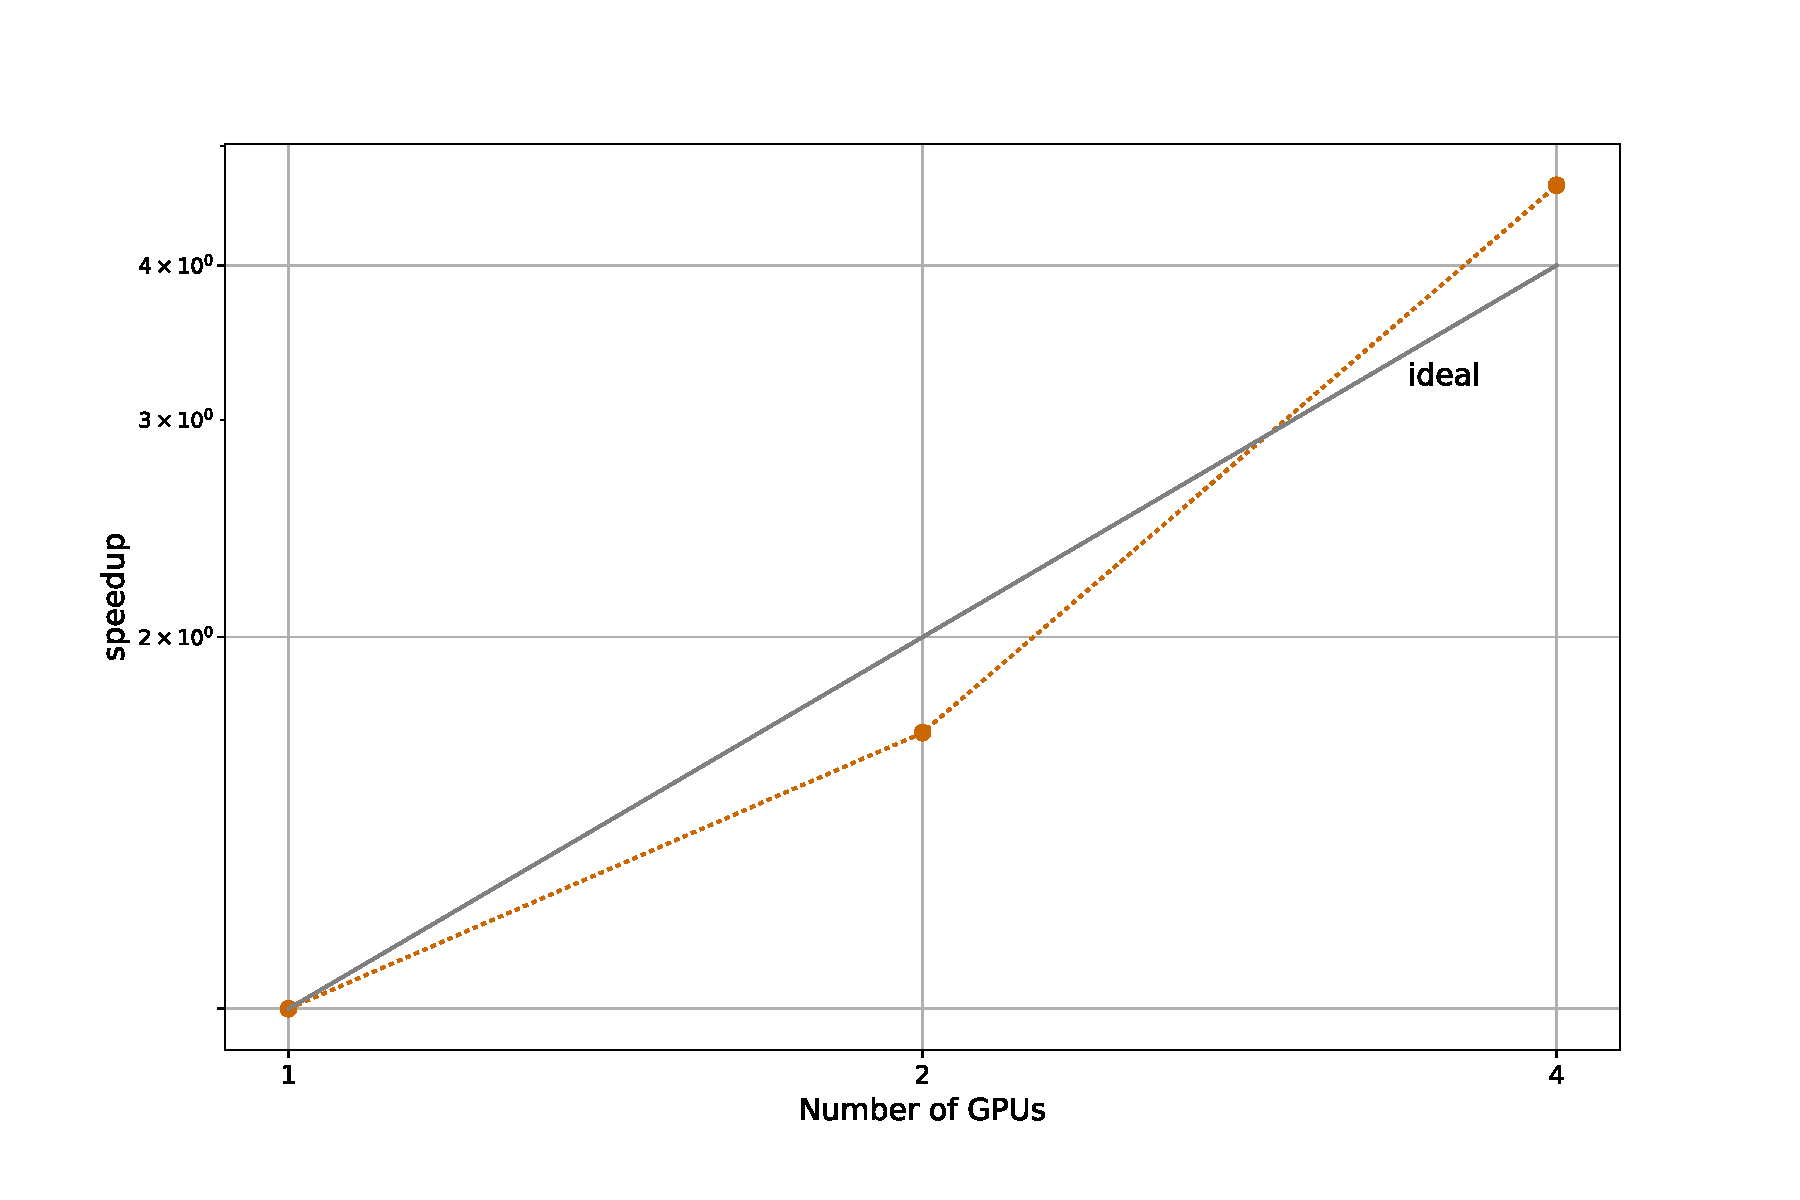
\includegraphics[width=.99\linewidth, clip, trim={1.5cm 1cm 2.5cm 2cm}]{strong-mpi.pdf}
		\caption{} 
		\label{fig:strong-mpi}
	\end{subfigure}%
	\begin{subfigure}{.5\textwidth}
		\centering
		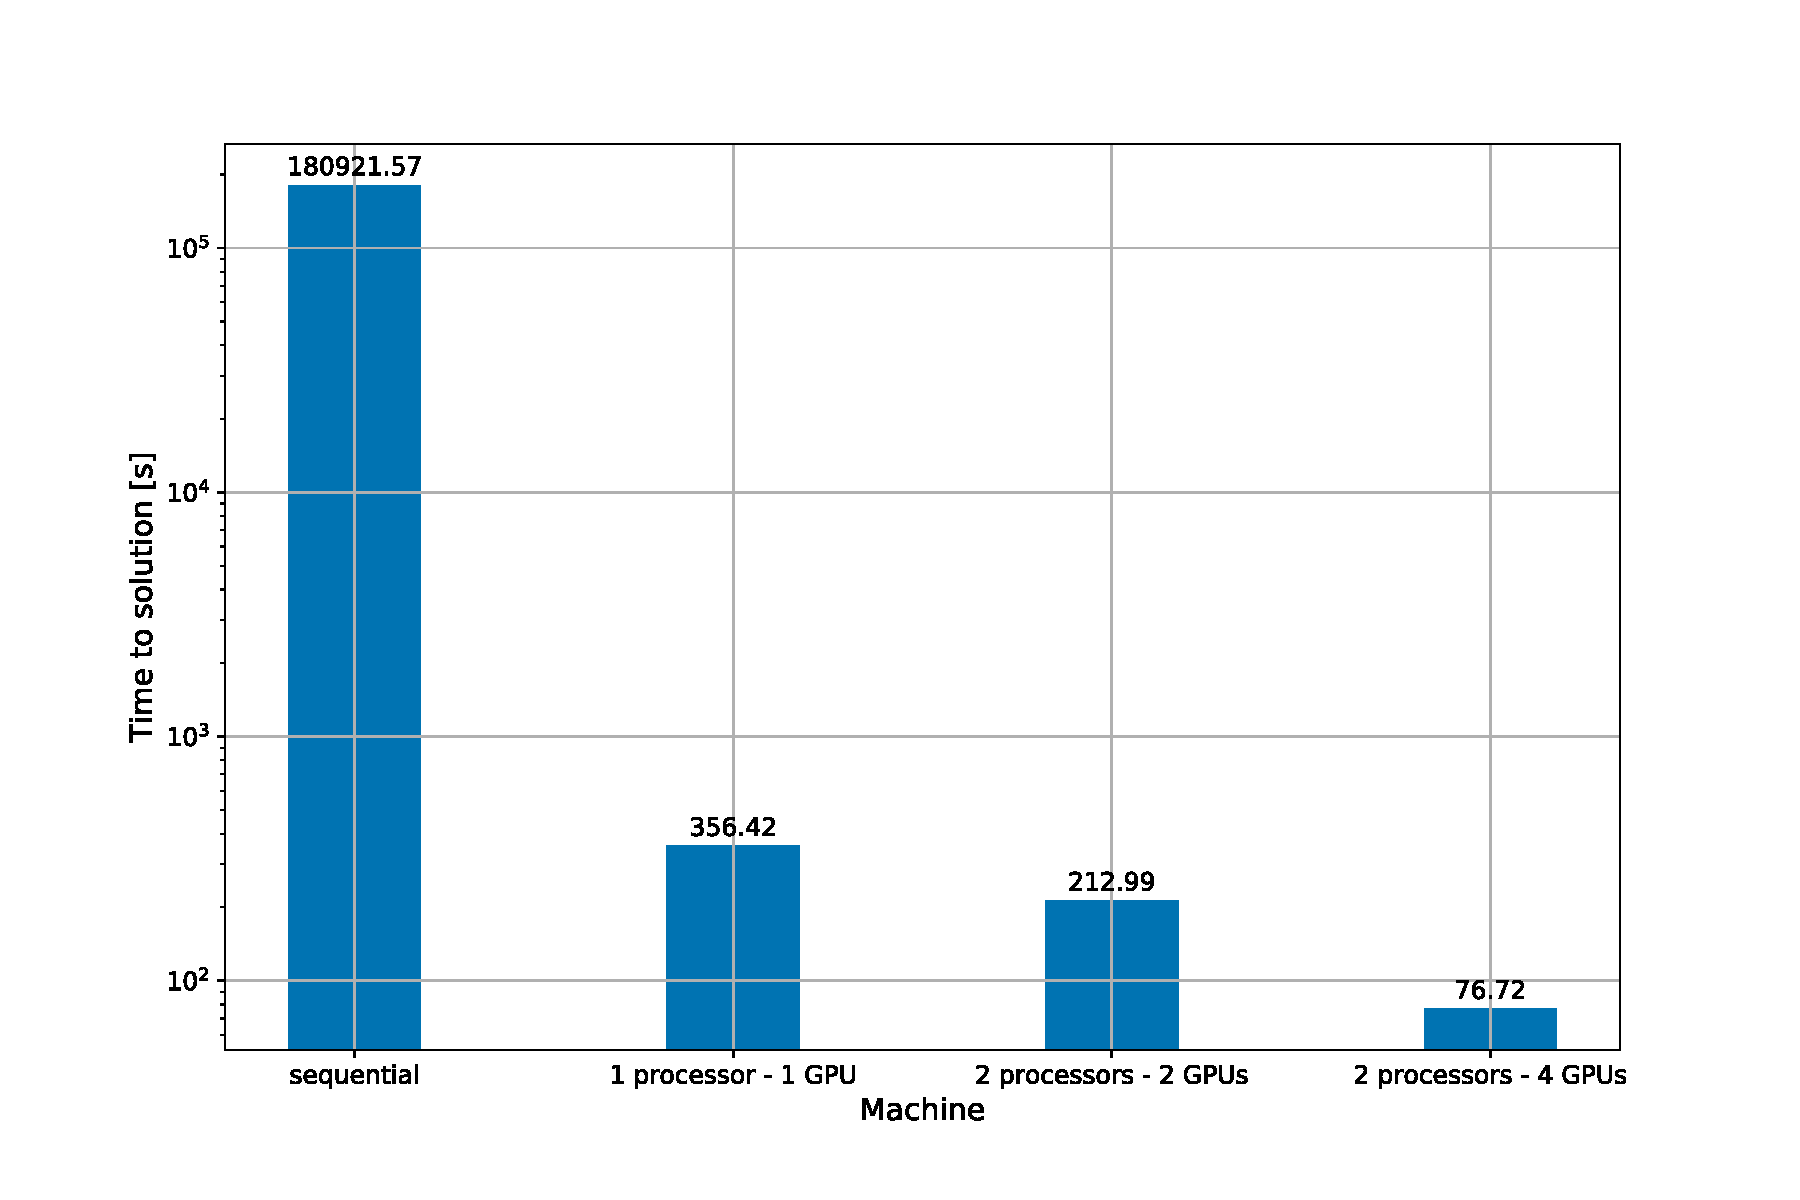
\includegraphics[width=.99\linewidth, clip, trim={1.5cm 1cm 2.5cm 2cm}]{strong-tts.pdf}
		\caption{} 
		\label{fig:strong-tts}
	\end{subfigure}
	\vspace{-0.4cm}
	\caption{Strong scaling as (a) the speedup for an increasing number of GPUs (via MPI) and (b) the reduced time to solution of the same problem ($25600\times14000$-pixel image, $max\_iteration=10,000,000$) for the different implementations.}
	\label{fig:strong}
\vspace{0.3cm}
\end{figure}

Finally, to evaluate the effect of weak scaling, we fix the image size to $368,640,000$ pixels and determine the value of $max\_iteration$ that allows each version to execute in around $76$ seconds.
The results are reported in the figure below.
\begin{figure}[H]
	\centering
	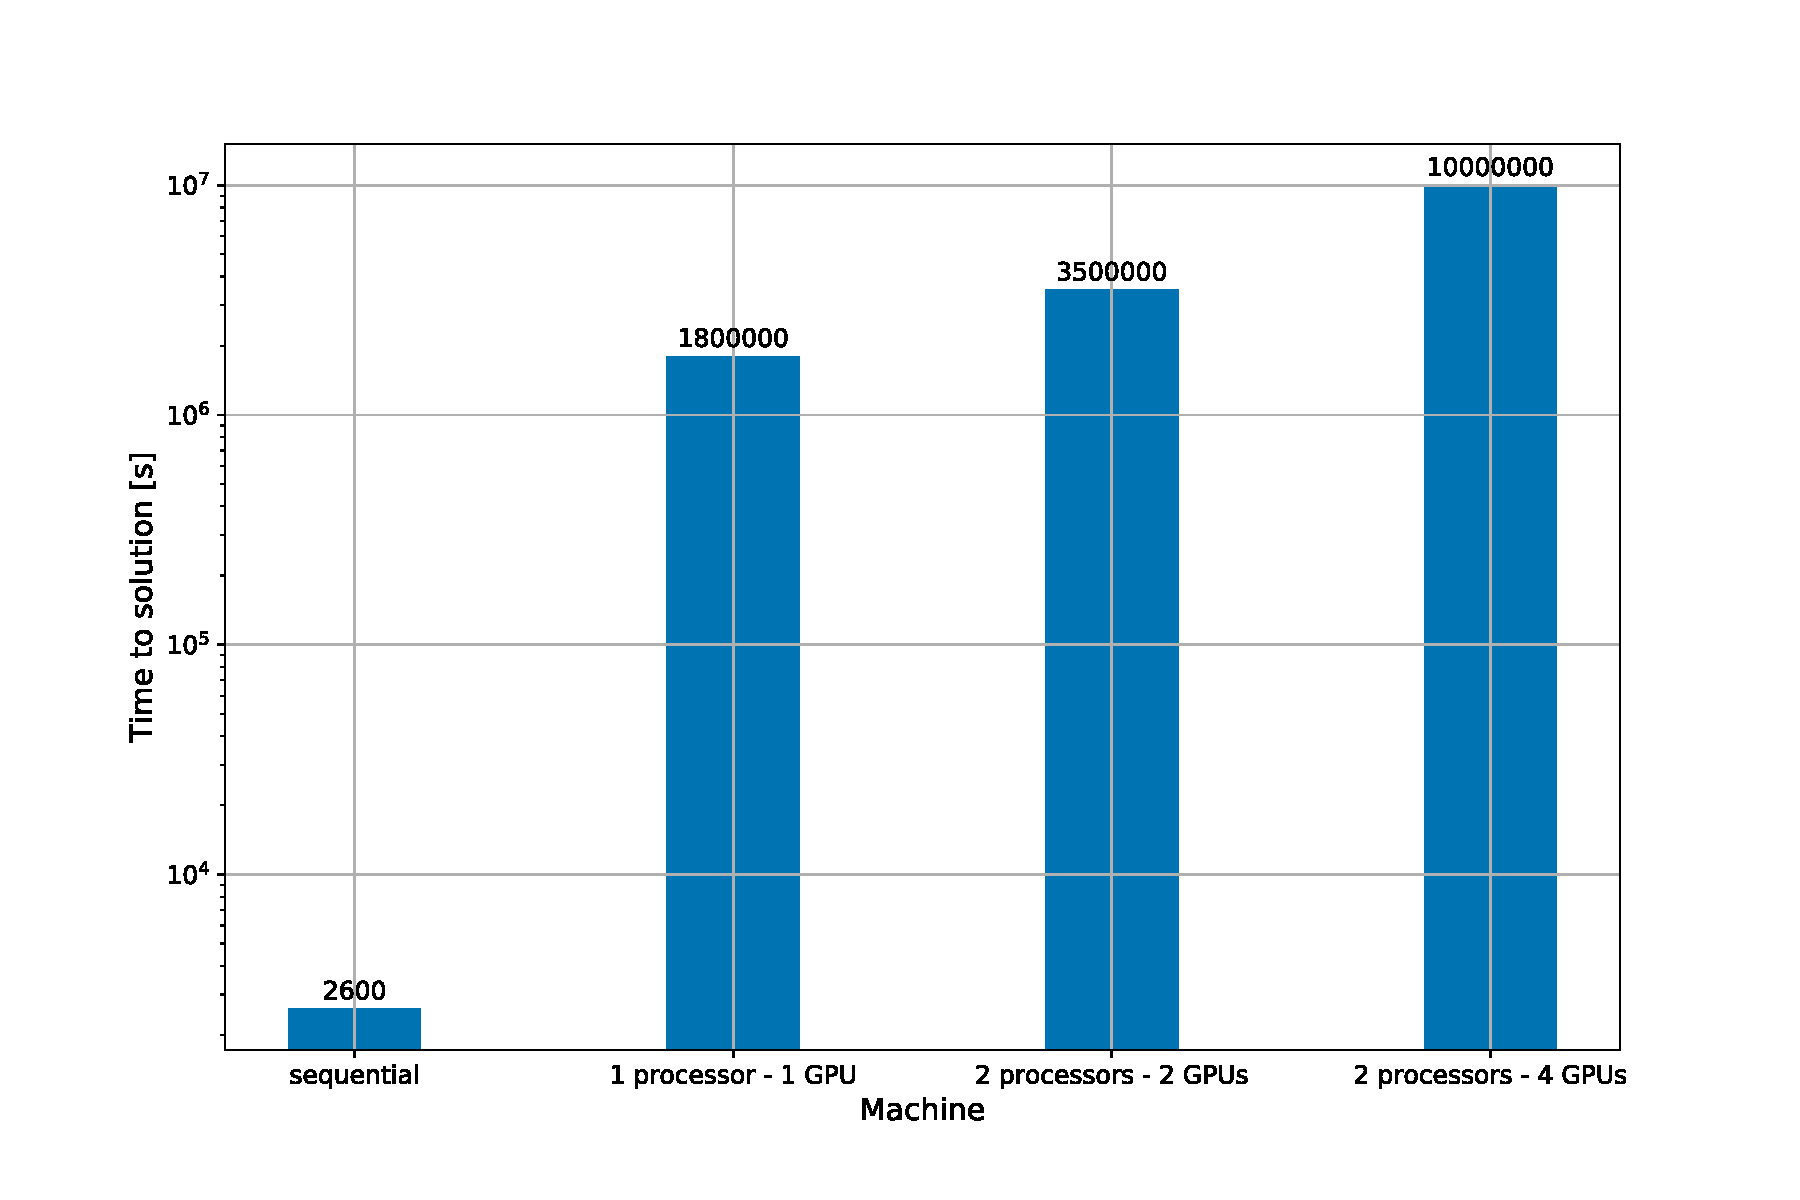
\includegraphics[width = 0.5\textwidth, clip, trim={1.5cm 1cm 2cm 2cm}]{weak.pdf}
	\caption{Weak scaling as a function of the problem size that can be solved in the same amount of time by the different implementations.}
	\label{fig:weak}
\end{figure}


\section{Resources budget}
\vspace{-0.1cm}
In order to fulfill the requirements of our project, we present hereafter the resource budget. 

\vspace{-0.2cm}
\subsection{Computing Power}
\vspace{-0.1cm}
The parallel implementations are compute-bound; hence, powerful GPUs are required.

\vspace{-0.2cm}
\subsection{Raw storage}
\vspace{-0.1cm}
The main requirement in terms of raw storage is due to the output images.
The largest image that we generate is $2.1~GB$.

\vspace*{-1cm}
\subsection{Grand Total}

\begin{center}
\begin{tabular}{| l | l |}
	\hline
	Total number of requested GPUs & 4\\
%	\hline
%	Minimum total memory & \textbf{\texttt{!! FIXME !!}} \\
%	\hline
%	Maximum total memory & \textbf{\texttt{!! FIXME !!}} \\
	\hline
	Temporary disk space for a single run & 3 GB \\
	\hline
	Permanent disk space for the entire project & 50 GB \\
	\hline
	Communications & MPI \\
	\hline
	License & MIT \\
	\hline
	Code publicly available ? & Yes \\
	\hline
	Library requirements & CUDA $\&$ MPI \\
	\hline
	Architectures where code ran & Deneb  \\
	\hline
\end{tabular}
\end{center}

\vspace{-0.3cm}
\section{Scientific outcome}
\vspace{-0.1cm}
The aim of this project is to gain experience and expertise on CUDA and MPI while developing applications in a supercomputer.
Throughout the development process, we have acquired familiarity with different tools for profiling and optimizing serial and parallel applications, as well as different technologies (such as non-blocking communications and parallel I/O in MPI).
All the skills that we have mastered in this context will constitute a fundamental basis for real submissions in larger high performance computing centers.


\vspace{-0.2cm}
\begin{thebibliography}{1}

\bibitem{wiki:mandelbrot} Wikipedia, {\em Mandelbrot set}, Online - accessed 09-May-2017, \url{https://en.wikipedia.org/wiki/Mandelbrot_set}\\[-17pt]

\bibitem{cuda} NVIDIA, {\em CUDA: Parallel Programming and Computing Platform}, Online - accessed 09-May-2017, \url{http://www.nvidia.com/object/cuda_home_new.html}\\[-17pt]

\bibitem{mpi} The MPI Forum, {\em MPI: A Message-Passing Interface Standard}, Technical Report, 1994\\[-17pt]

\bibitem{ritchie} Kernighan, Brian W. and Ritchie, Dennis M., {\em The C Programming Language Second Edition}, Prentice-Hall, Inc.,1988\\[-17pt]

\bibitem{smooth} Stack Overflow, {\em Improvement to my Mandelbrot set code}, Online - accessed 09-May-2017, \url{http://stackoverflow.com/questions/16124127/improvement-to-my-mandelbrot-set-code}\\[-17pt]

\bibitem{scitas} Scientific IT and Application Support, {\em Deneb and its extension, Eltanin}, Online - accessed 14-May-2017, \url{http://scitas.epfl.ch/hardware/deneb-and-eltanin}\\[-17pt]

\bibitem{costs} Vincent Hindriksen, {\em How expensive is an operation on a CPU?}, Online - accessed 14-May-2017, \url{https://streamcomputing.eu/blog/2012-07-16/how-expensive-is-an-operation-on-a-cpu/}\\[-17pt]

%\bibitem{if} Stack Overflow, {\em Is “IF” expensive?}, Online - accessed 14-May-2017,
%\url{http://stackoverflow.com/questions/315306/is-if-expensive}\\[-17pt]

\bibitem{gpus} NVIDIA, {\em NVIDIA TESLA GPU ACCELERATORS}, Online - accessed 1-June-2017,
\url{http://www.nvidia.com/content/tesla/pdf/nvidia-tesla-kepler-family-datasheet.pdf}\\[-17pt]

\bibitem{guide} NVIDIA, {\em CUDA C Programming Guide}, Online - accessed 1-June-2017,
\url{http://docs.nvidia.com/cuda/cuda-c-programming-guide/#axzz4j1NpsHeT}\\[-17pt]

\bibitem{occupancy} NVIDIA, {\em CUDA Warps and Occupancy}, Online - accessed 1-June-2017,
\url{http://on-demand.gputechconf.com/gtc-express/2011/presentations/cuda_webinars_WarpsAndOccupancy.pdf}

\end{thebibliography}


\end{document}
